%% (Master) Thesis template
% Template version used: v1.4
%
% Largely adapted from Adrian Nievergelt's template for the ADPS
% (lecture notes) project.


%% We use the memoir class because it offers a many easy to use features.
\documentclass[11pt,a4paper,titlepage]{memoir}

%% Packages
%% ========

%% LaTeX Font encoding -- DO NOT CHANGE
\usepackage[OT1]{fontenc}

%% Babel provides support for languages.  'english' uses British
%% English hyphenation and text snippets like "Figure" and
%% "Theorem". Use the option 'ngerman' if your document is in German.
%% Use 'american' for American English.  Note that if you change this,
%% the next LaTeX run may show spurious errors.  Simply run it again.
%% If they persist, remove the .aux file and try again.
\usepackage[english]{babel}

%% Input encoding 'utf8'. In some cases you might need 'utf8x' for
%% extra symbols. Not all editors, especially on Windows, are UTF-8
%% capable, so you may want to use 'latin1' instead.
\usepackage[utf8]{inputenc}



%% This changes default fonts for both text and math mode to use Herman Zapfs
%% excellent Palatino font.  Do not change this.
\usepackage[sc]{mathpazo}

%% The AMS-LaTeX extensions for mathematical typesetting.  Do not
%% remove.
\usepackage{amsmath,amssymb,amsfonts,mathrsfs}

%% NTheorem is a reimplementation of the AMS Theorem package. This
%% will allow us to typeset theorems like examples, proofs and
%% similar.  Do not remove.
%% NOTE: Must be loaded AFTER amsmath, or the \qed placement will
%% break
\usepackage[amsmath,thmmarks]{ntheorem}

%% LaTeX' own graphics handling
\usepackage{graphicx}

%% We unfortunately need this for the Rules chapter.  Remove it
%% afterwards; or at least NEVER use its underlining features.
\usepackage{soul}

%% This allows you to add .pdf files. It is used to add the
%% declaration of originality.
\usepackage{pdfpages}

%% Some more packages that you may want to use.  Have a look at the
%% file, and consult the package docs for each.
%% See the TeXed file for more explanations
%% [REC] Format dates and time depending on locale
\usepackage{datetime}

%% [OPT] Multi-rowed cells in tabulars
%\usepackage{multirow}

%% [REC] Intelligent cross reference package. This allows for nice
%% combined references that include the reference and a hint to where
%% to look for it.

\usepackage{varioref}

%% [OPT] Easily changeable quotes with \enquote{Text}
%\usepackage[german=swiss]{csquotes}



%% [OPT] Provides a \cancel{} command to stroke through mathematics.
%\usepackage{cancel}

%% [NEED] This allows for additional typesetting tools in mathmode.
%% See its excellent documentation.
\usepackage{mathtools}

%% [ADV] Conditional commands
%\usepackage{ifthen}

%% [OPT] Manual large braces or other delimiters.
%\usepackage{bigdelim, bigstrut}

%% [REC] Alternate vector arrows. Use the command \vv{} to get scaled
%% vector arrows.
\usepackage[h]{esvect}

%% [NEED] Some extensions to tabulars and array environments.
\usepackage{array}

%% [OPT] Postscript support via pstricks graphics package. Very
%% diverse applications.
%\usepackage{pstricks,pst-all}

%% [?] This seems to allow us to define some additional counters.
%\usepackage{etex}

%% [ADV] XY-Pic to typeset some matrix-style graphics
%\usepackage[all]{xy}

%% [OPT] This is needed to generate an index at the end of the
%% document.
%\usepackage{makeidx}

%% [OPT] Fancy package for source code listings.  The template text
%% needs it for some LaTeX snippets; remove/adapt the \lstset when you
%% remove the template content.
\usepackage{listings}
\lstset{language=TeX,basicstyle={\normalfont\ttfamily}}

%% [REC] Fancy character protrusion.  Must be loaded after all fonts.
\usepackage[activate]{pdfcprot}

%% [REC] Nicer tables.  Read the excellent documentation.
\usepackage{booktabs}

%% lmodern removes this restriction by allowing font sizes at arbitrary sizes
\usepackage{lmodern}


%% Our layout configuration.  DO NOT CHANGE.
%% Memoir layout setup

%% NOTE: You are strongly advised not to change any of them unless you
%% know what you are doing.  These settings strongly interact in the
%% final look of the document.

% Dependencies
\usepackage{UNIGElogo}

% Turn extra space before chapter headings off.
\setlength{\beforechapskip}{0pt}

\nonzeroparskip
\parindent=0pt
\defaultlists

% Chapter style redefinition
\makeatletter

\if@twoside
  \pagestyle{Ruled}
  \copypagestyle{chapter}{Ruled}
\else
  \pagestyle{ruled}
  \copypagestyle{chapter}{ruled}
\fi
\makeoddhead{chapter}{}{}{}
\makeevenhead{chapter}{}{}{}
\makeheadrule{chapter}{\textwidth}{0pt}
\copypagestyle{abstract}{empty}

\makechapterstyle{bianchimod}{%
  \chapterstyle{default}
  \renewcommand*{\chapnamefont}{\normalfont\Large\sffamily}
  \renewcommand*{\chapnumfont}{\normalfont\Large\sffamily}
  \renewcommand*{\printchaptername}{%
    \chapnamefont\centering\@chapapp}
  \renewcommand*{\printchapternum}{\chapnumfont {\thechapter}}
  \renewcommand*{\chaptitlefont}{\normalfont\huge\sffamily}
  \renewcommand*{\printchaptertitle}[1]{%
    \hrule\vskip\onelineskip \centering \chaptitlefont\textbf{\vphantom{gyM}##1}\par}
  \renewcommand*{\afterchaptertitle}{\vskip\onelineskip \hrule\vskip
    \afterchapskip}
  \renewcommand*{\printchapternonum}{%
    \vphantom{\chapnumfont {9}}\afterchapternum}}

% Use the newly defined style
\chapterstyle{bianchimod}

\setsecheadstyle{\Large\bfseries\sffamily}
\setsubsecheadstyle{\large\bfseries\sffamily}
\setsubsubsecheadstyle{\bfseries\sffamily}
\setparaheadstyle{\normalsize\bfseries\sffamily}
\setsubparaheadstyle{\normalsize\itshape\sffamily}
\setsubparaindent{0pt}

% Set captions to a more separated style for clearness
\captionnamefont{\sffamily\bfseries\footnotesize}
\captiontitlefont{\sffamily\footnotesize}
\setlength{\intextsep}{16pt}
\setlength{\belowcaptionskip}{1pt}

% Set section and TOC numbering depth to subsection
\setsecnumdepth{subsection}
\settocdepth{subsection}

%% Titlepage adjustments
\pretitle{\vspace{10pt plus 0.7fill}\begin{center}\HUGE\sffamily\bfseries}
\posttitle{\end{center}\par}
\preauthor{\par\begin{center}\let\and\\\Large\sffamily}
\postauthor{\end{center}}
\predate{\par\begin{center}\Large\sffamily}
\postdate{\end{center}}

\def\@advisors{}
\newcommand{\advisors}[1]{\def\@advisors{#1}}
\def\@department{}
\newcommand{\department}[1]{\def\@department{#1}}
\def\@thesistype{}
\newcommand{\thesistype}[1]{\def\@thesistype{#1}}

\renewcommand{\maketitlehooka}{\noindent\UNIGElogo[3in]}

\renewcommand{\maketitlehookb}{\vspace{1in}%
  \par\begin{center}\Large\sffamily\@thesistype\end{center}}

\renewcommand{\maketitlehookd}{%
  \vfill\par
  \begin{flushright}
    \sffamily
    \@advisors\par
    \@department, UNIGE Geneva
  \end{flushright}
}

\checkandfixthelayout

\setlength{\droptitle}{-48pt}

\makeatother

% This defines how theorems should look. Best leave as is.
\theoremstyle{plain}
\setlength\theorempostskipamount{0pt}

%%% Local Variables:
%%% mode: latex
%%% TeX-master: "thesis"
%%% End:


%% Theorem environments.  You will have to adapt this for a German
%% thesis.
%% Theorem-like environments

%% This can be changed according to language. You can comment out the ones you
%% don't need.

\numberwithin{equation}{chapter}

%% German theorems
%\newtheorem{satz}{Satz}[chapter]
%\newtheorem{beispiel}[satz]{Beispiel}
%\newtheorem{bemerkung}[satz]{Bemerkung}
%\newtheorem{korrolar}[satz]{Korrolar}
%\newtheorem{definition}[satz]{Definition}
%\newtheorem{lemma}[satz]{Lemma}
%\newtheorem{proposition}[satz]{Proposition}

%% English variants
\newtheorem{theorem}{Theorem}[chapter]
\newtheorem{example}[theorem]{Example}
\newtheorem{remark}[theorem]{Remark}
\newtheorem{corollary}[theorem]{Corollary}
\newtheorem{definition}[theorem]{Definition}
\newtheorem{lemma}[theorem]{Lemma}
\newtheorem{proposition}[theorem]{Proposition}

%% Proof environment with a small square as a "qed" symbol
\theoremstyle{nonumberplain}
\theorembodyfont{\normalfont}
\theoremsymbol{\ensuremath{\square}}
\newtheorem{proof}{Proof}
%\newtheorem{beweis}{Beweis}


%% Helpful macros.
%% Custom commands
%% ===============

%% Special characters for number sets, e.g. real or complex numbers.
\newcommand{\C}{\mathbb{C}}
\newcommand{\K}{\mathbb{K}}
\newcommand{\N}{\mathbb{N}}
\newcommand{\Q}{\mathbb{Q}}
\newcommand{\R}{\mathbb{R}}
\newcommand{\Z}{\mathbb{Z}}
\newcommand{\X}{\mathbb{X}}

%% Fixed/scaling delimiter examples (see mathtools documentation)
\DeclarePairedDelimiter\abs{\lvert}{\rvert}
\DeclarePairedDelimiter\norm{\lVert}{\rVert}

%% Use the alternative epsilon per default and define the old one as \oldepsilon
\let\oldepsilon\epsilon
\renewcommand{\epsilon}{\ensuremath\varepsilon}

%% Also set the alternate phi as default.
\let\oldphi\phi
\renewcommand{\phi}{\ensuremath{\varphi}}


%%% citation 
%\usepackage{cite}
%\usepackage[authoryear, sort, square]{natbib}

%% color text
\usepackage{xcolor}

%% Highlighted text color
\usepackage{soul}



%% Make document internal hyperlinks wherever possible. (TOC, references)
%% This MUST be loaded after varioref, which is loaded in 'extrapackages'
%% above.  We just load it last to be safe.
\usepackage[linkcolor=black,colorlinks=true,citecolor=black,filecolor=black]{hyperref}
%\usepackage{textcomp}
\newcommand{\MONTH}{%
	\ifcase\the\month
	\or January% 1
	\or February% 2
	\or March% 3
	\or April% 4
	\or May% 5
	\or June% 6
	\or July% 7
	\or August% 8
	\or September% 9
	\or October% 10
	\or November% 11
	\or December% 12
	\fi}
\makeatletter
\newcommand{\YEAR}{\@Roman{\the\year}}
% Copyrigthed symbole
%\DeclareTextCommandDefault{\textcopyright}{\textcircled{c}}

\usepackage{subcaption}
\usepackage{wrapfig}
\usepackage{sidecap}
\usepackage{float}
%% Document information
%% ====================

%\advisors{Advisors: Prof.\ Dr.\ A. D. Visor, Dr.\ P. Ostdoc}
\date{September 01, 2017}
\title{\Large\textsc{Strategies for Digital Documentation of Maker Projects}}
\author{M. O. Darwich}
\thesistype{State-of-the-Art}
%\advisors{Advisors: Prof.\ Dr.\ A. D. Visor, Dr.\ P. Ostdoc}
\condition{\centering Submitted to the \textit{Department of Computer Science} in partial fulfilment of the requirements for the course \\ \Large{\textbf{Design Science Research}} \\
\textcopyright Mohammad Oday Darwich, \YEAR, All rights reserved}
\department{\vfill Department of Computer Science}
\date{August 17, 2017}

\begin{document}

\frontmatter

%% Title page is autogenerated from document information above.  DO
%% NOT CHANGE.
\begin{titlingpage}
  \calccentering{\unitlength}
  \begin{adjustwidth*}{\unitlength-24pt}{-\unitlength-24pt}
    \maketitle
  \end{adjustwidth*}

\end{titlingpage}

%% The abstract of your thesis.  Edit the file as needed.
%\begin{abstract}
  This example thesis briefly shows the main features of our thesis
  style, and how to use it for your purposes.
\end{abstract}


%% TOC with the proper setup, do not change.
\cleartorecto
\tableofcontents
\mainmatter

%% Your real content!
% Some commands used in this file
\newcommand{\package}{\emph}

\chapter{Introduction}



\chapter{Platform analyses} 


\section{Instructable}


\begin{center}
	\begin{minipage}{.7\textwidth}
		\textit{In this section, I share with you an analyses of how users create and share \textit{DIY} projects via online platform called Instructables. I share findings of the analyses of this platform and the understanding of how authors and users use Instructables}
	\end{minipage}
\end{center}

\begin{comment}
\hl{What is it ?} \hl{Who use it ?} \hl{User interactions ?} \hl{Limitations} \hl{Advantages ?} \hl{Examples ?} \\
\end{comment}

\begin{figure}[ht!]
	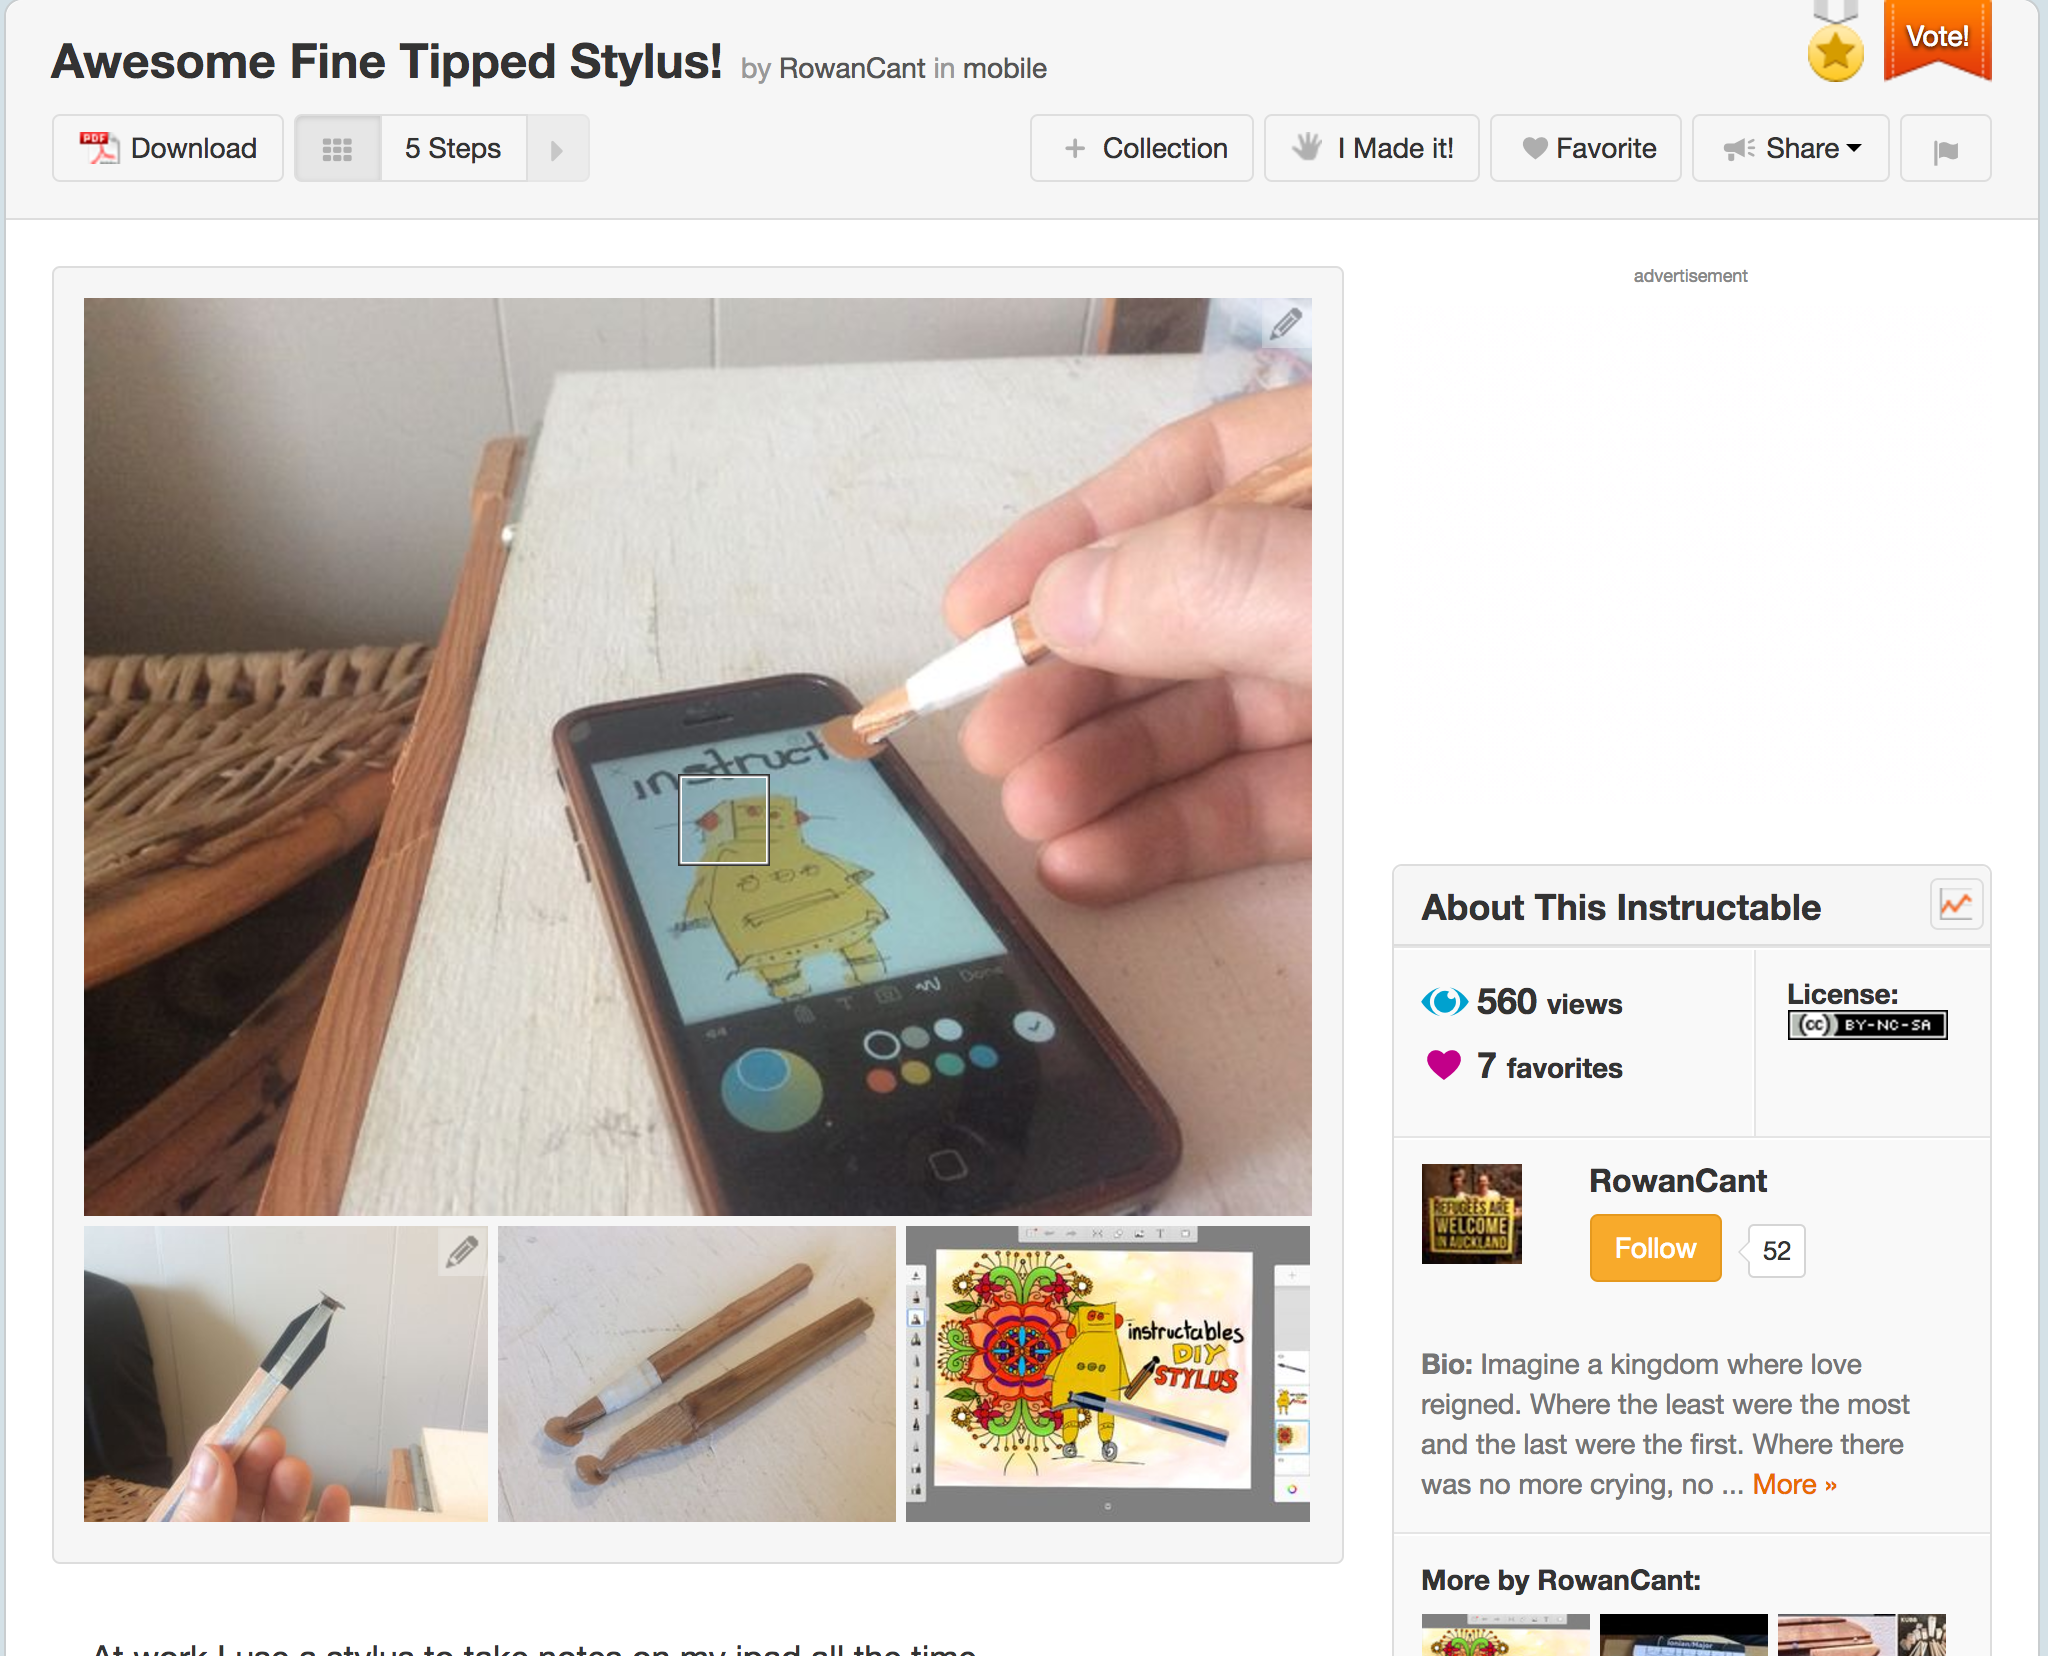
\includegraphics[scale=0.36]{./images/img-instructables.png}
	\caption{Sample Instructables project, \url{http://www.instructables.com/id/Awesome-Fine-Tipped-Stylus/}}
	\label{sec:img-instructables}
\end{figure}

Instructables is an online platform for \textit{DIY} communities that serves as a "place that lets you explore, document, and share your creations" \cite{web:instructable}. It is a website specializing in user-created and uploaded do-it-yourself projects, which other users can comment on and rate for quality \cite{wiki:instructable} \cite{wiki:instructable}. There are different categories of project such as technology, crafts, food, home, workshops and living, with more than 263,258 projects and 9,888,442 monthly visit as of August 2017. Users create their project step by step and with each step they describe what they did in a text, photos or videos as displayed in the figure \ref{sec:img-instructables}. The encapsulation of steps produce a typical guide that help others to re-create the project, learn from it or build a new thing on top of it and have their own version of the project. 

The contributions in Instructables come from the sharing culture of projects, not only authors contribute but also readers who can view and give feedback by commenting on the project. Also, Instructables create a social community where they exchange their thoughts about a topic via forums and subforms dedicated to a special topic such as Arduino projects. Finally, prizes are given to the top shared Instructables as a kind of reward for their effort of sharing their project and to keep them connected with the community.

\subsection{Methodology} 

To understand the users interactions of Instructables, an extensive study of the Instructables community has been done in the fall of 2011, this study used semi-structured interviews and online surveys. The semi-structured interviews had a framework of four themes that had been explored : (\oldstylenums{1}) motivation, (\oldstylenums{2}) Documentation tools, (\oldstylenums{3}) Writing an Instructable and (\oldstylenums{4}) Feedback. A theme was covered by a set of questions that took one hour with each interviewer. \cite{scholar:Tseng:2014:PVP:2598510.2598540}. A survey of 15 multiple-choice questions and open ended-questions that ask users about different aspects of their experience with replicating or building on top of a project shared by a user on the platform.

\subsection{User interaction}

The study has shown three strategies for documenting a project. The first was to \textit{write after you make}, as shown in the figure \ref{img-writemake}  \cite{tseng2016making}.
\begin{figure}[ht!]
	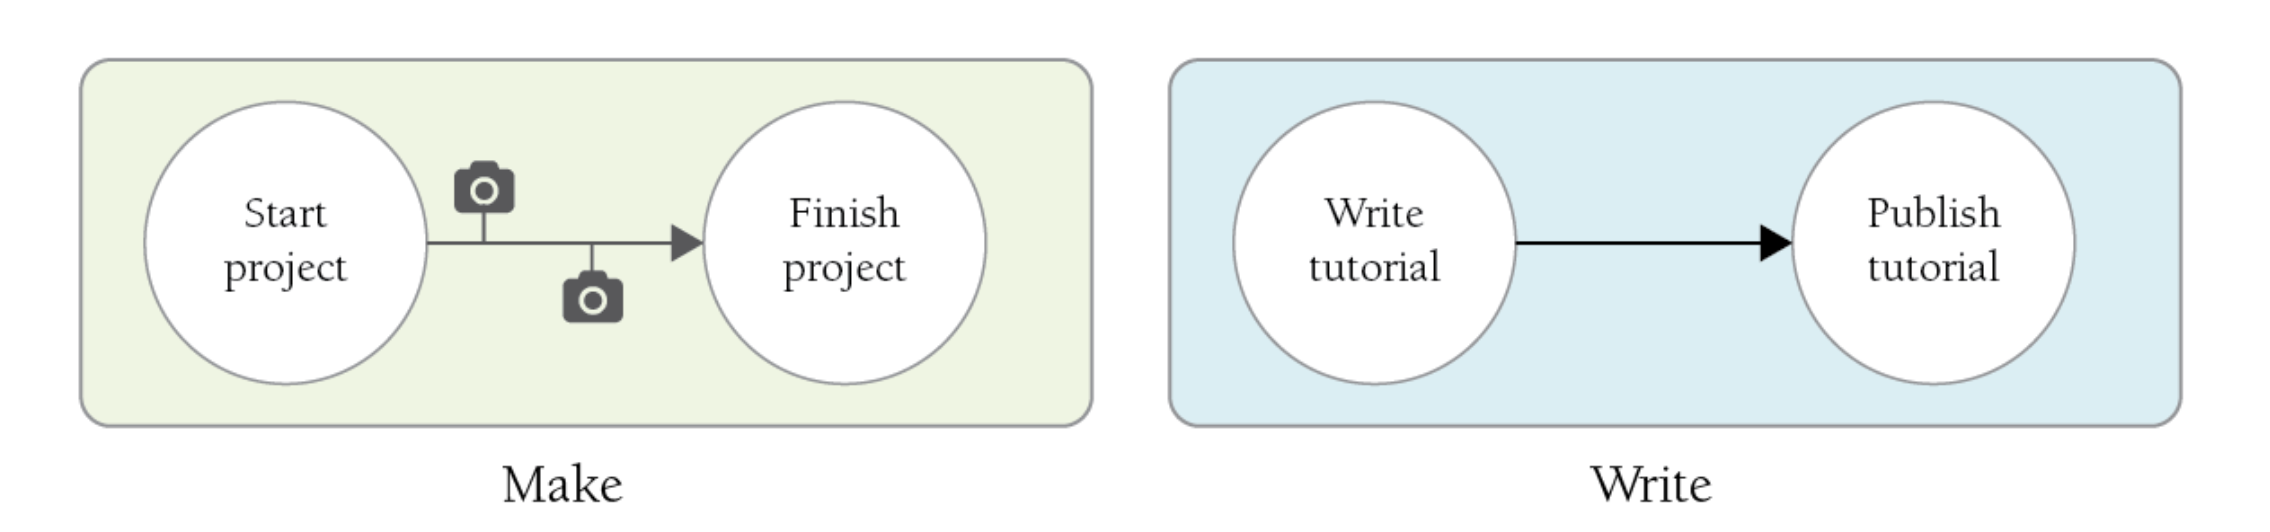
\includegraphics[scale=0.34]{./images/img-writemake.png}
	\caption{First strategy of documenting : write after you make, \cite{tseng2016making}}
	\label{img-writemake}
\end{figure}

A problem confronted the users with this strategy, users forgot to document in the midst of making. Users outperformed this problem by following the second strategy of \textit{writing after replicating}, as displayed in the figure \ref{img-makereplicatewrite} \cite{scholar:Tseng:2014:PVP:2598510.2598540}
\begin{figure}[ht!]
	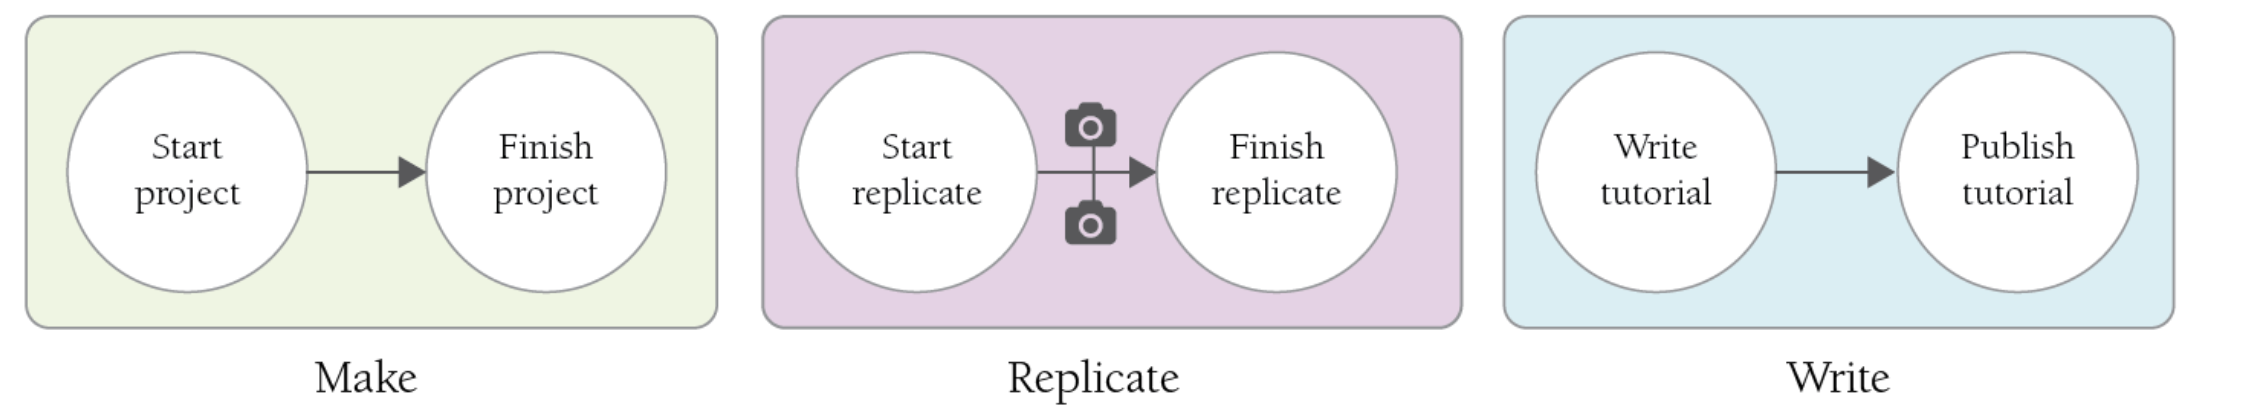
\includegraphics[scale=0.34]{./images/img-makereplicatewrite.png}
	\caption{First strategy of documenting : Make, replicate  then write, \cite{tseng2016making}}
	\label{img-makereplicatewrite}
\end{figure}

The final strategy was to \textit{simultaneously write and make} (figure \ref{img-makewritesimultanously}). 
\begin{figure}[ht!]
	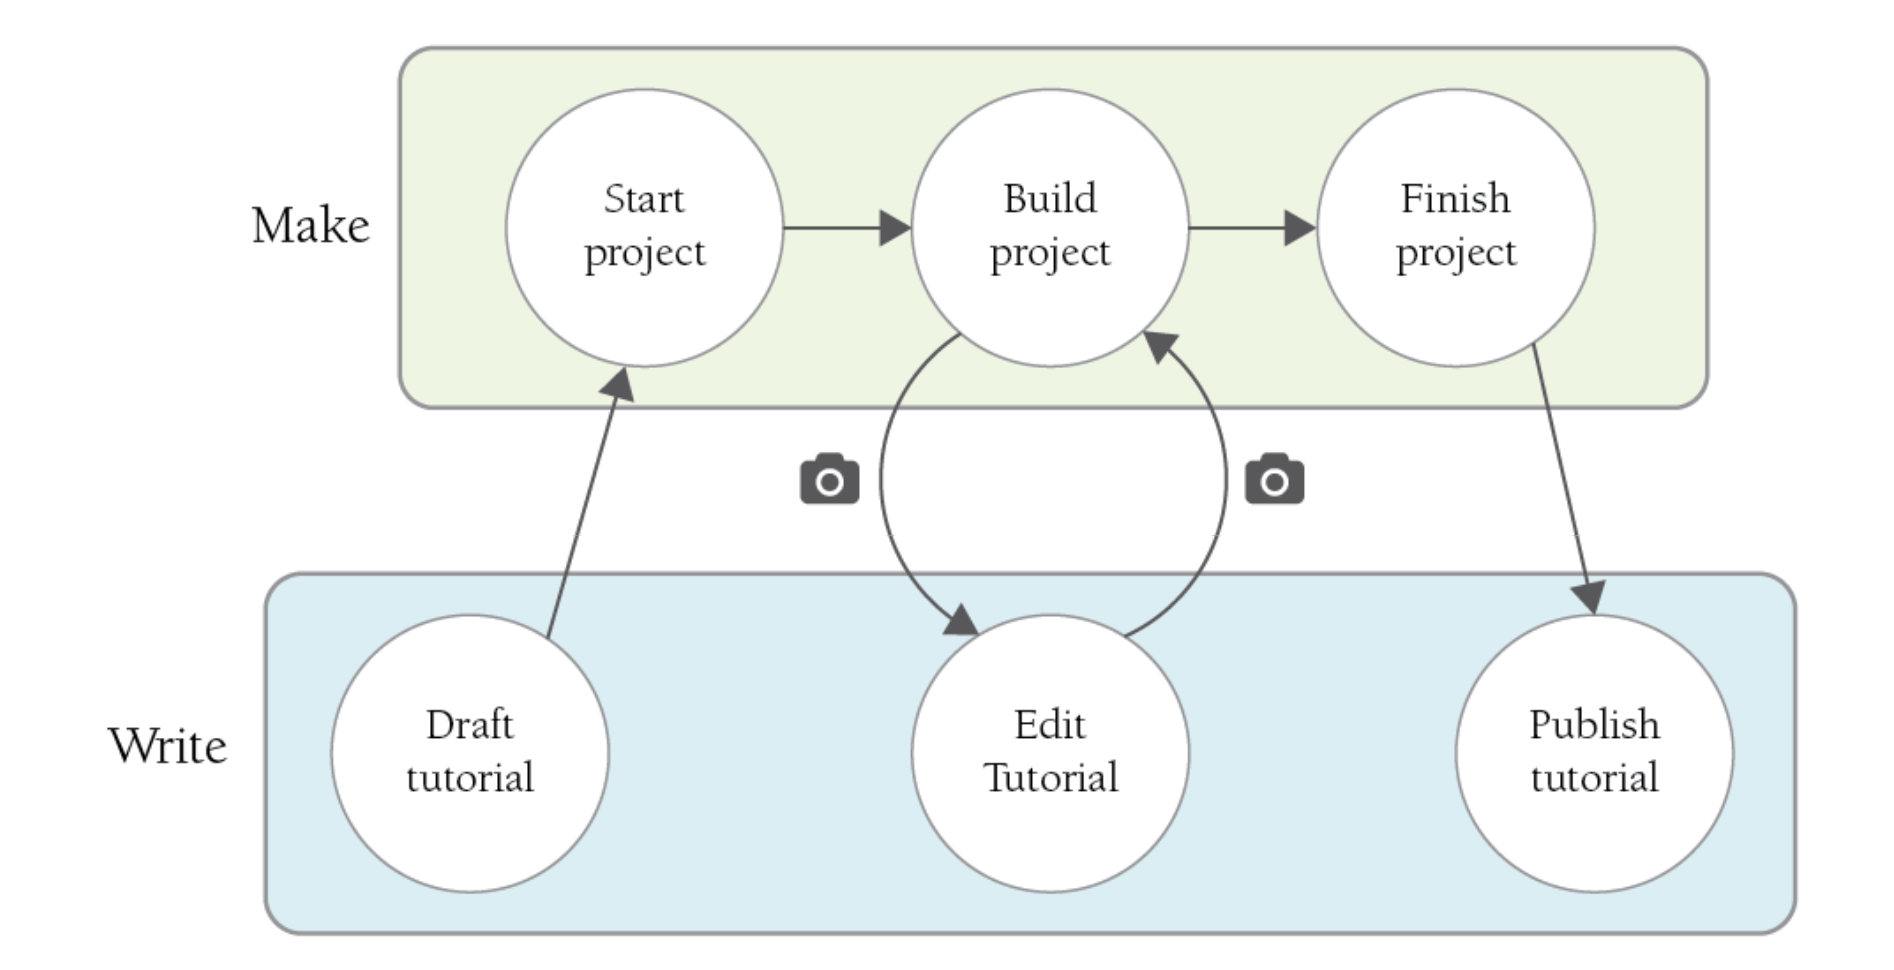
\includegraphics[scale=0.34]{./images/img-makewritesimultanously}
	\caption{First strategy of documenting : write after you make, \cite{tseng2016making}}
	\label{img-makewritesimultanously}
\end{figure}

In summary, the study showed that users need to encapsulate the collected photos and videos to show to create all the steps and a common challenge was to remember to document after each step otherwise users had to replicate their project merely to creating good documentation. 

Finally, authors saw that documentation well worth the effort to share their work but it is time consuming process when a project get more complex, it is hard to follow up or complete the documentation. \cite{scholar:Wakkary:2015:TAH:2702123.2702550}

\subsection{Design and process oriented documentation}
Several approaches were suggested by to improve the online documentation. Documentation techniques requires authors to simultaneously switch between making and writing, make a design process to not miss a step from not being documented or to radically recreate the project to document it in a proper way. Another challenges of documentation technique that needed to support not only the capture of digital artifacts but also physical artifacts where it is not possible to show the physical effort. 
With the recurring need to balance manual and automated ways of capturing, software and hardware tools need to solve open questions and be customizable for different activities and different audiences \cite{Kuznetsov:2010:REA:1868914.1868950}. The workflow of documentation over time needed to not miss a key step in the documentation. 

Documentation process seems to be more important for readers as it give them the opportunity to enable better decision making about components or materials to use \cite{scholar:sf1241364}, as well as successful in encouraging independent exploration and fostering a sense of accomplishment \cite{scholar:lovell2010sewing}. Also, as many users start by replicating some projects, having tools where they could be able to contribute to a project, can help more socializing and boost a collaborative work in the community. 

\section{Build In Progress}
%\hl{What is it ?} \hl{Who use it ?} \hl{User interactions ?} \hl{Limitations} \hl{Advantages ?} \hl{Examples ?}

Build in Progress is a platform for sharing the story of your design process, where \textit{"makers share how their DIY projects evolve over time}" \cite{tseng2016making}. It focus more on the storytelling of \textit{DIY} documented project, a snapshot of the platform displayed in the figure \ref{img-buildinprogress}.

BiP was launched in 2013 and within a collaboration with many institutions and a network of schools, it hosted over 1368 projects in categories such as Electronics, Mechanical and living. Users contributed to BiP community by sharing, providing feedback and describing their progress of each step, the encapsulation of informations lead to a story about the project as BiP "\textit{support a storytelling approach to documentation}" \cite{tseng2016making}.
\begin{figure}[ht!]
	\centering
	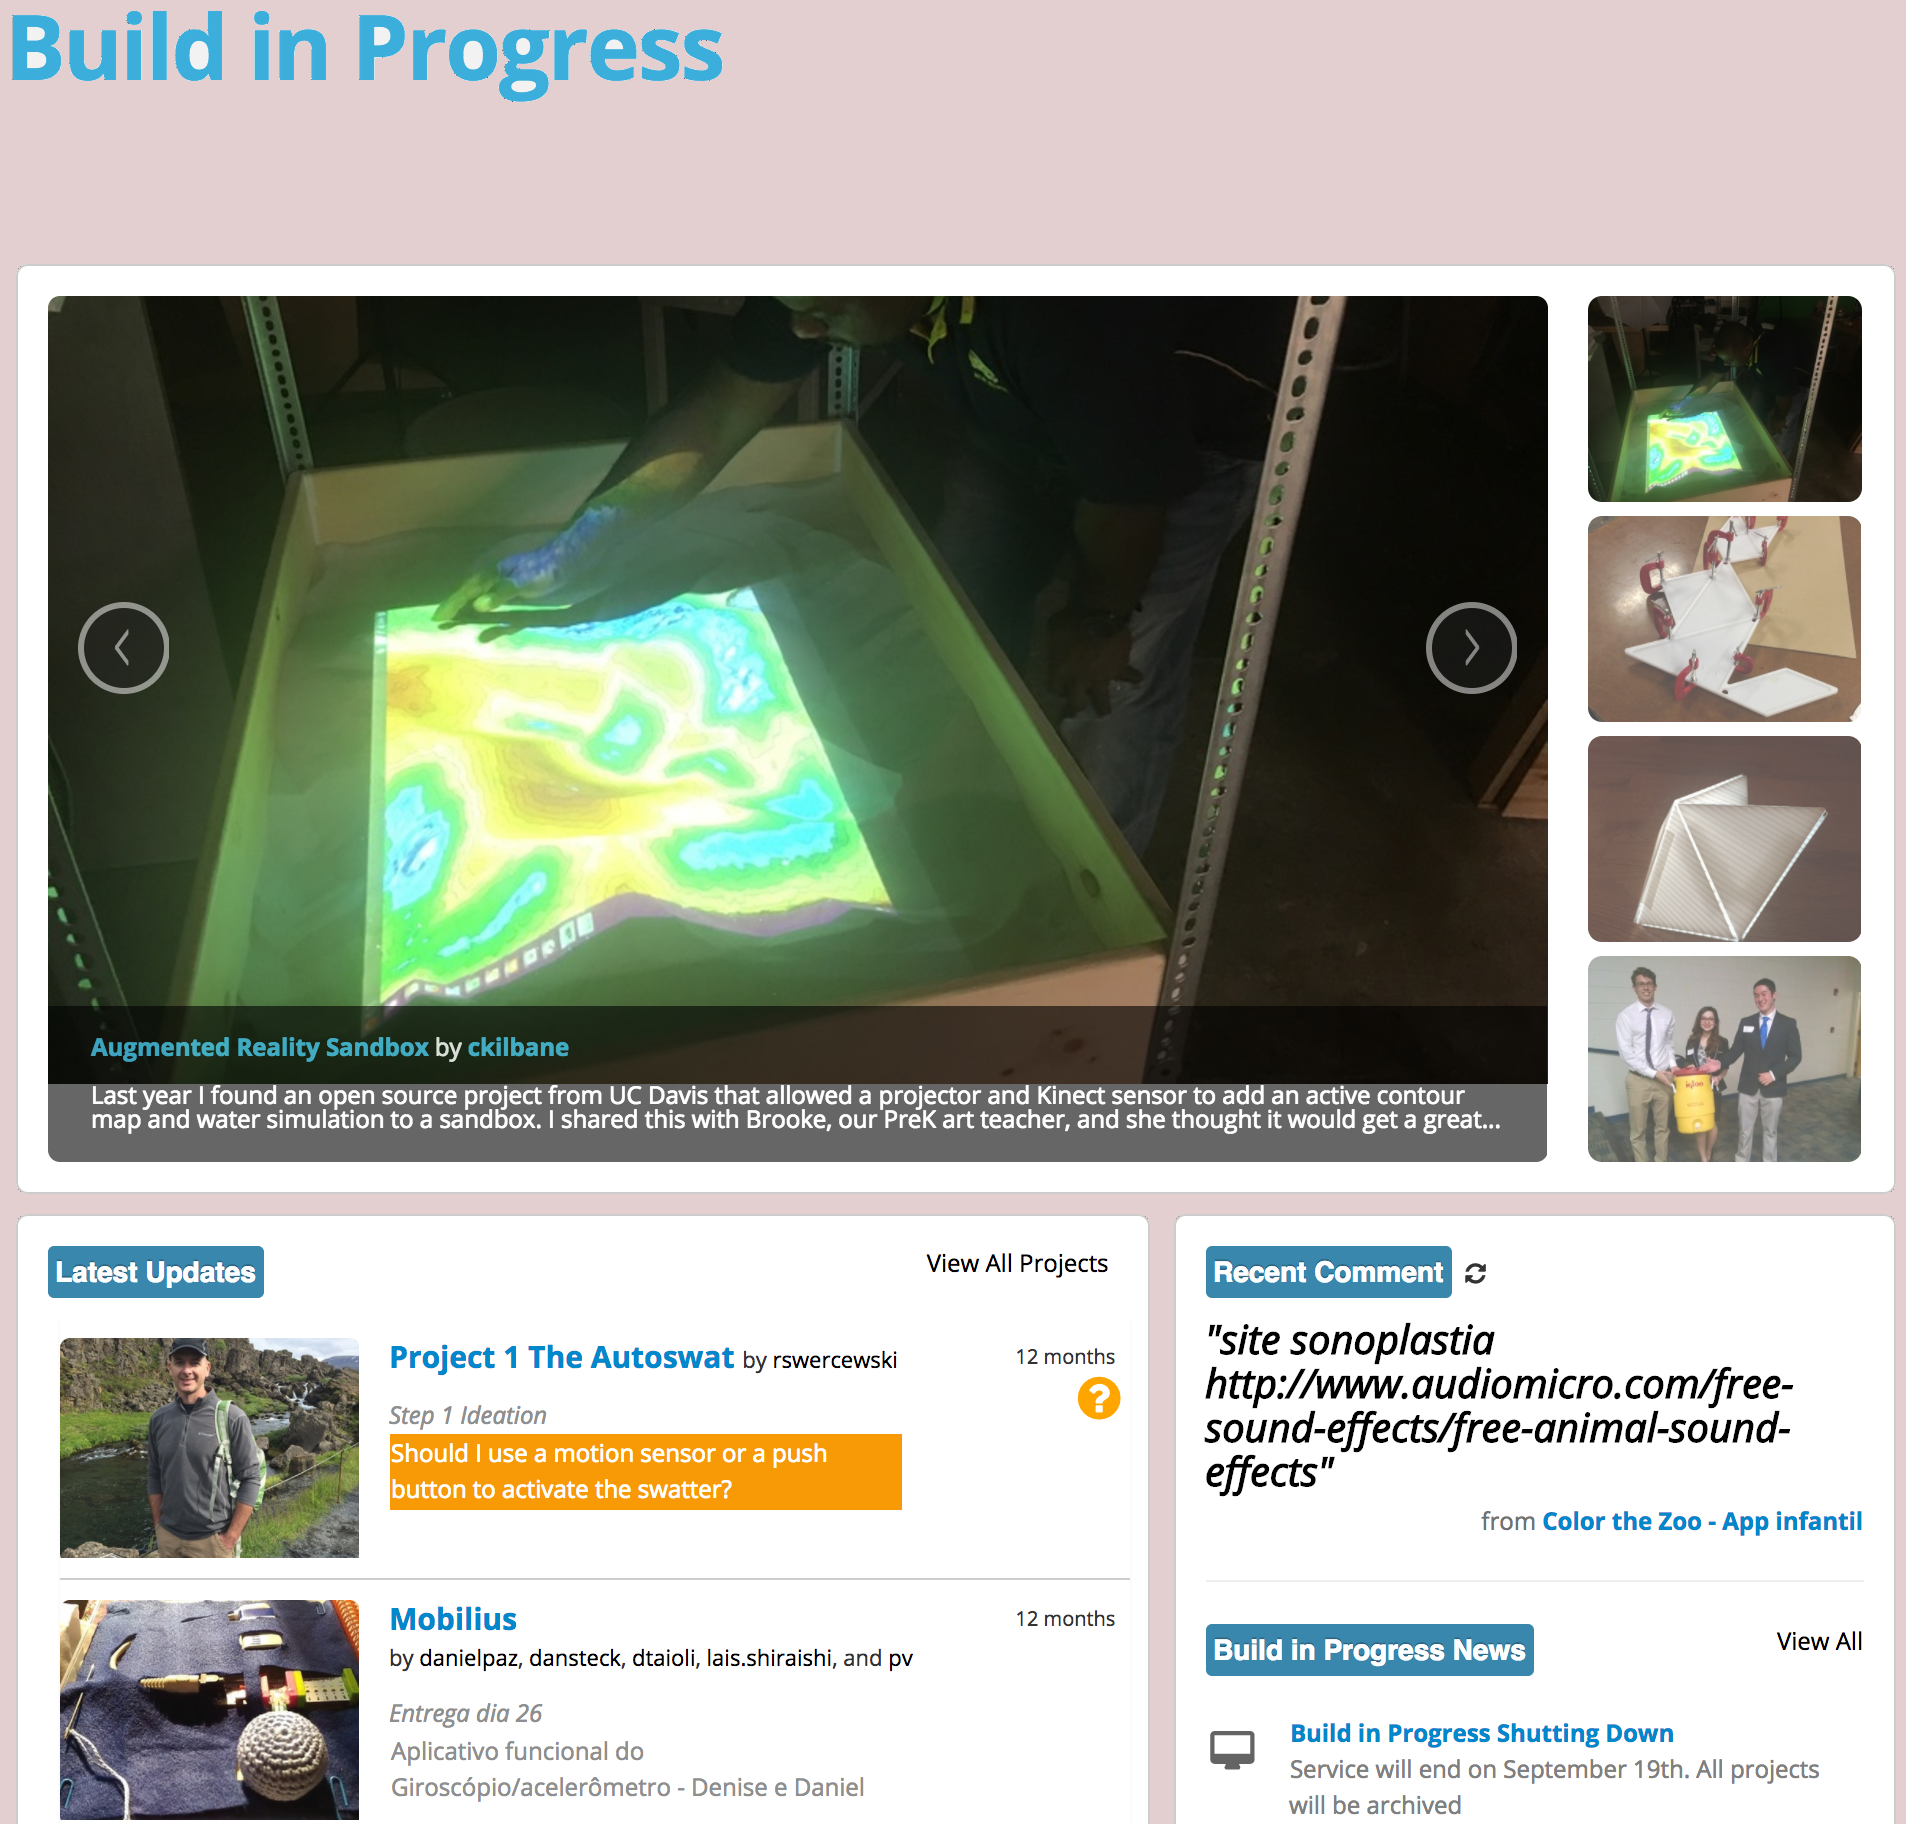
\includegraphics[width=10cm, height=10cm]{./images/img-buildinprogress.png}
	\caption{Build in progress welcome page, \cite{BuildinP1}} 
	\label{img-buildinprogress}
\end{figure}

\vspace{-1cm}
\subsection{Design approach}
Authors shared an iterative design process in the context of sharing their personal journey by creating step-by-step instructions of their project via the online platform \textit{BiP} and companion mobile application. Readers contributed by suggesting to makers after publishing their steps, makers benefited from sharing step-by-step instructions over time by taking into account the suggestions of readers.

BiP was developed based on an innovative design process, it enables users to visualize their documentation in an iterative way. Authors can continuously iterate their building process, share their techniques to help others to reach out others in the community so they can have feedback. A social design process principle was considered among the online community to engage users more, to accumulate knowledge, to learn from others and connect users with same interest as \textit{human-related issues in the form of social ties and knowledge sharing were reported as keys to successful collaboration} \cite{Kotlarsky2005}.

\subsection{Features}\label{sec:feature}
BiP consists of many features in the project page and social feature. The two core features of the project page are : the \textit{Process Map} and \textit{Step Detail View } (\ref{img-bipprojectpage}).
\begin{figure}[ht!]
	\centering
	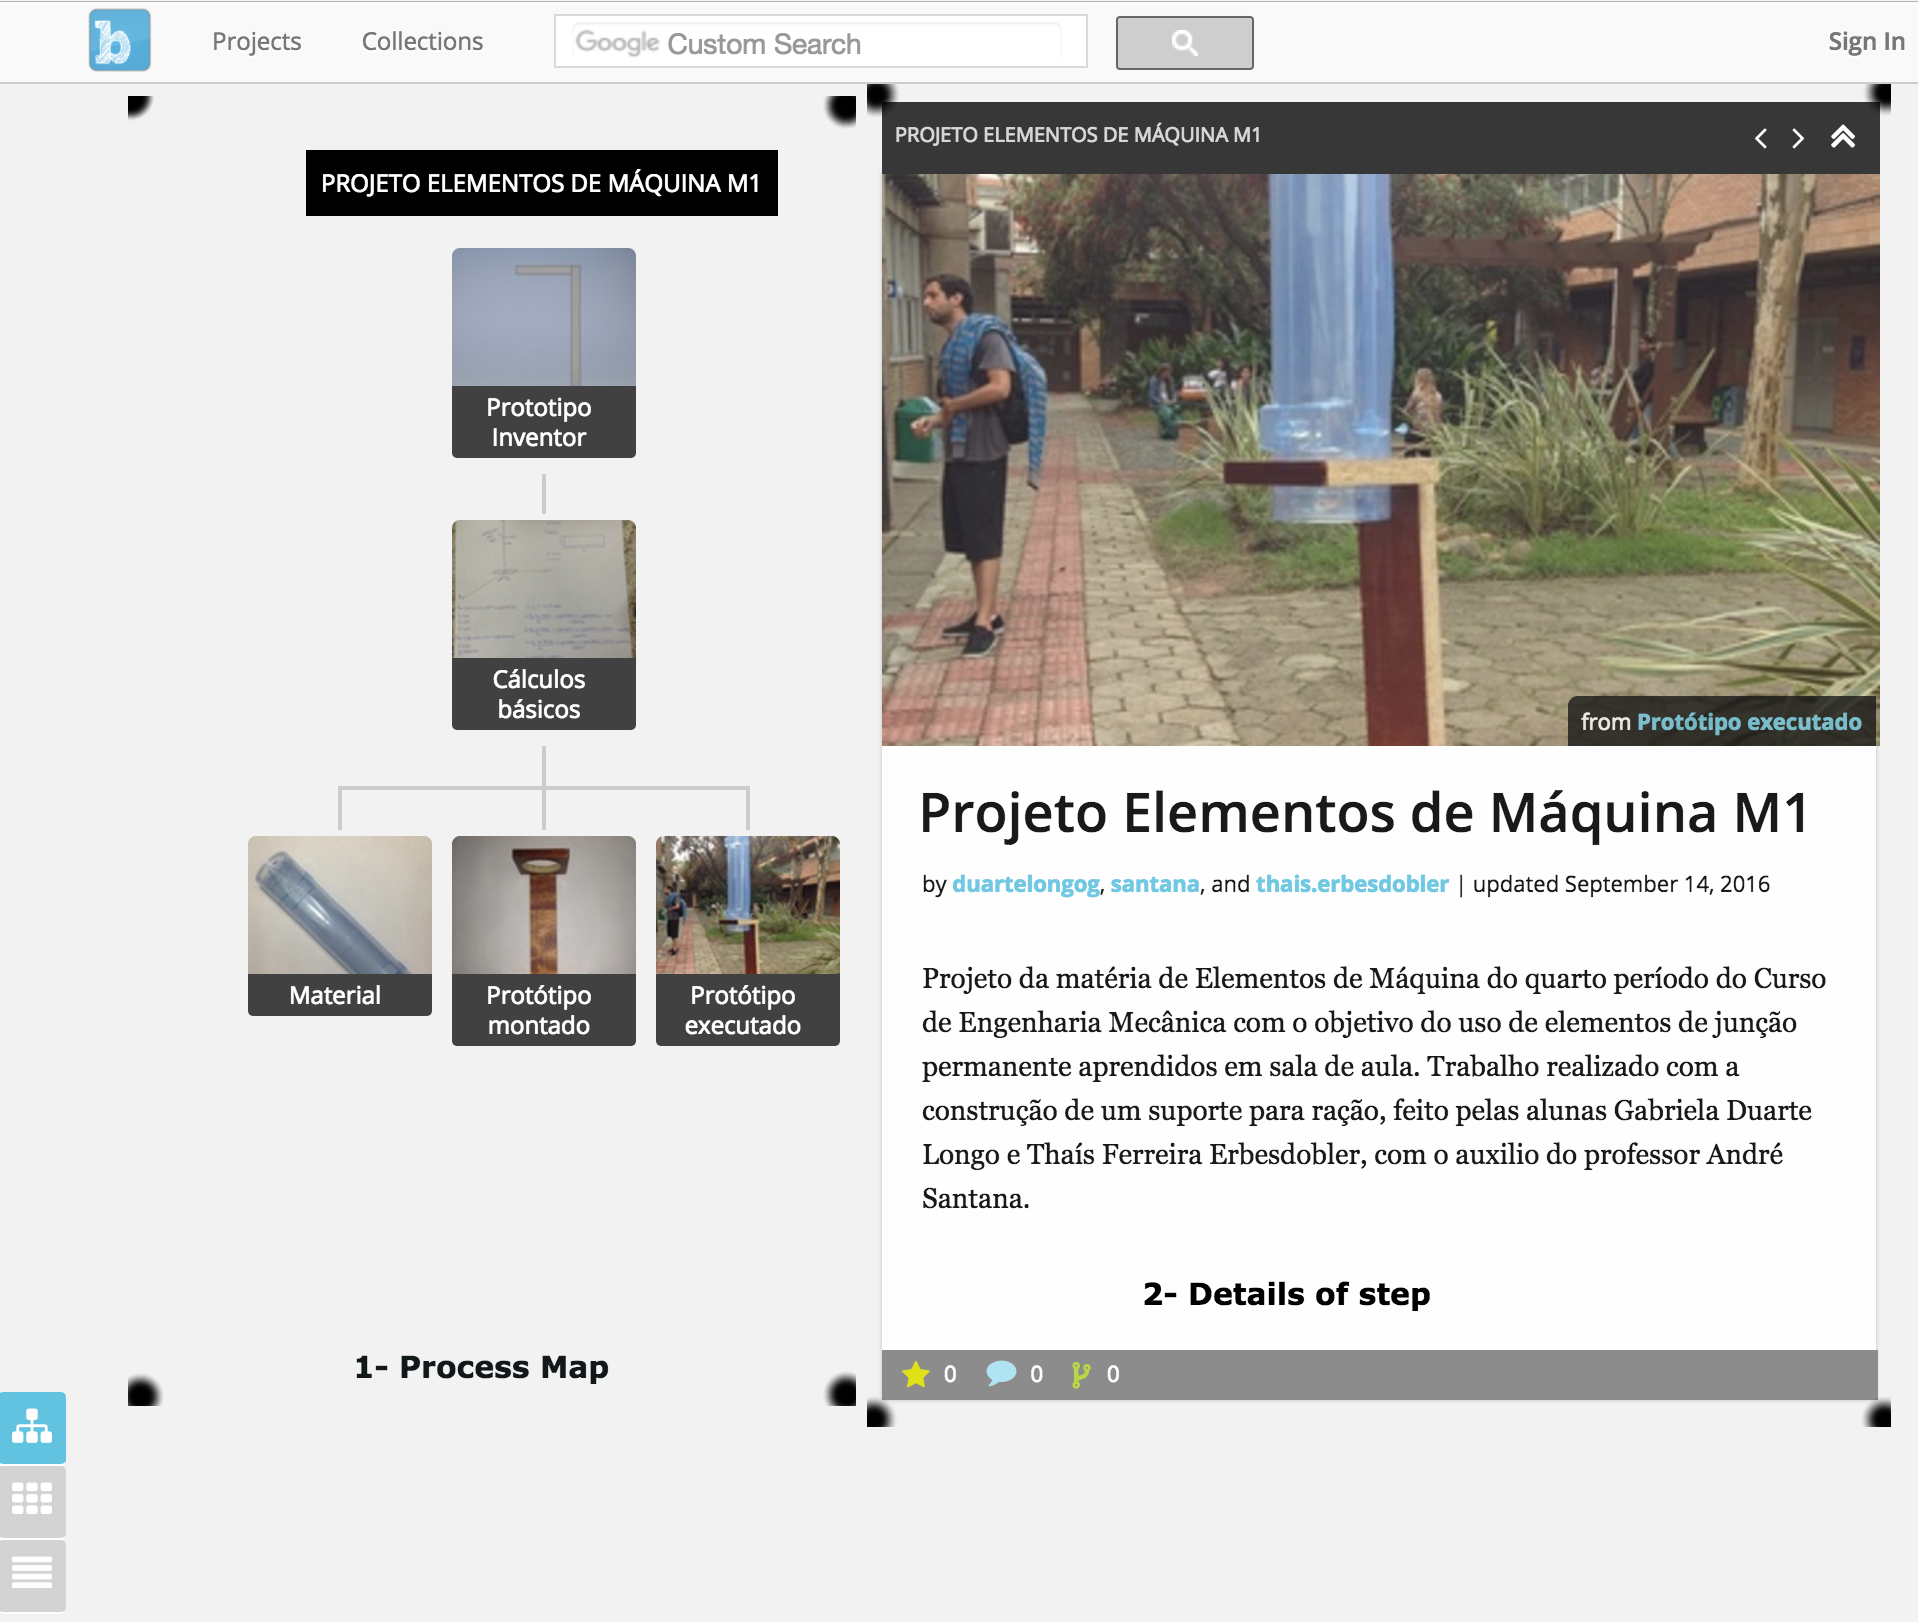
\includegraphics[width=.3\textheight]{./images/img-bipprojectpage.png}
	\caption{overall project view, \cite[\url{http://buildinprogress.media.mit.edu/projects/4599/steps}]{BuildinP1}} 
	\label{img-bipprojectpage}
\end{figure}
In the process map, users can create a step, a label for one or more step, drag \& drop  to rearrange steps. Steps are organized in a tree-map-like format with sui generis branches, a label is added to a branch and it can be colored to designate a branch; for example orange labels represent that a branch is in progress.

Project are displayed in 3 different mode.  The first is the default mode : tree-map, users can go through all the steps, step-by-step and discover more about it as shown in figure \ref{img-mode1}.
\begin{figure}[H]
	\centering
	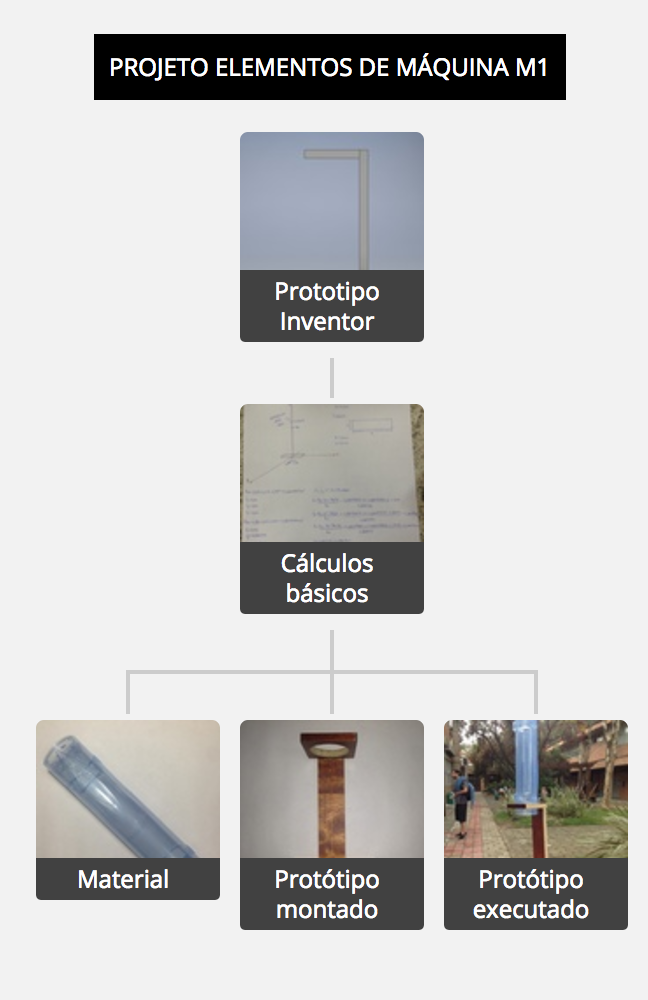
\includegraphics[scale=.3]{./images/img-mode1.png}
	\caption{tree-map view of the project} 
	\label{img-mode1}
\end{figure}

The second is Gallery mode \ref{img-mode2} and finally  the  blog mode : users can scroll down and an index of steps will be displayed on their left side of the page (figure \ref{img-mode3}).

\begin{figure}[H]
	\centering
	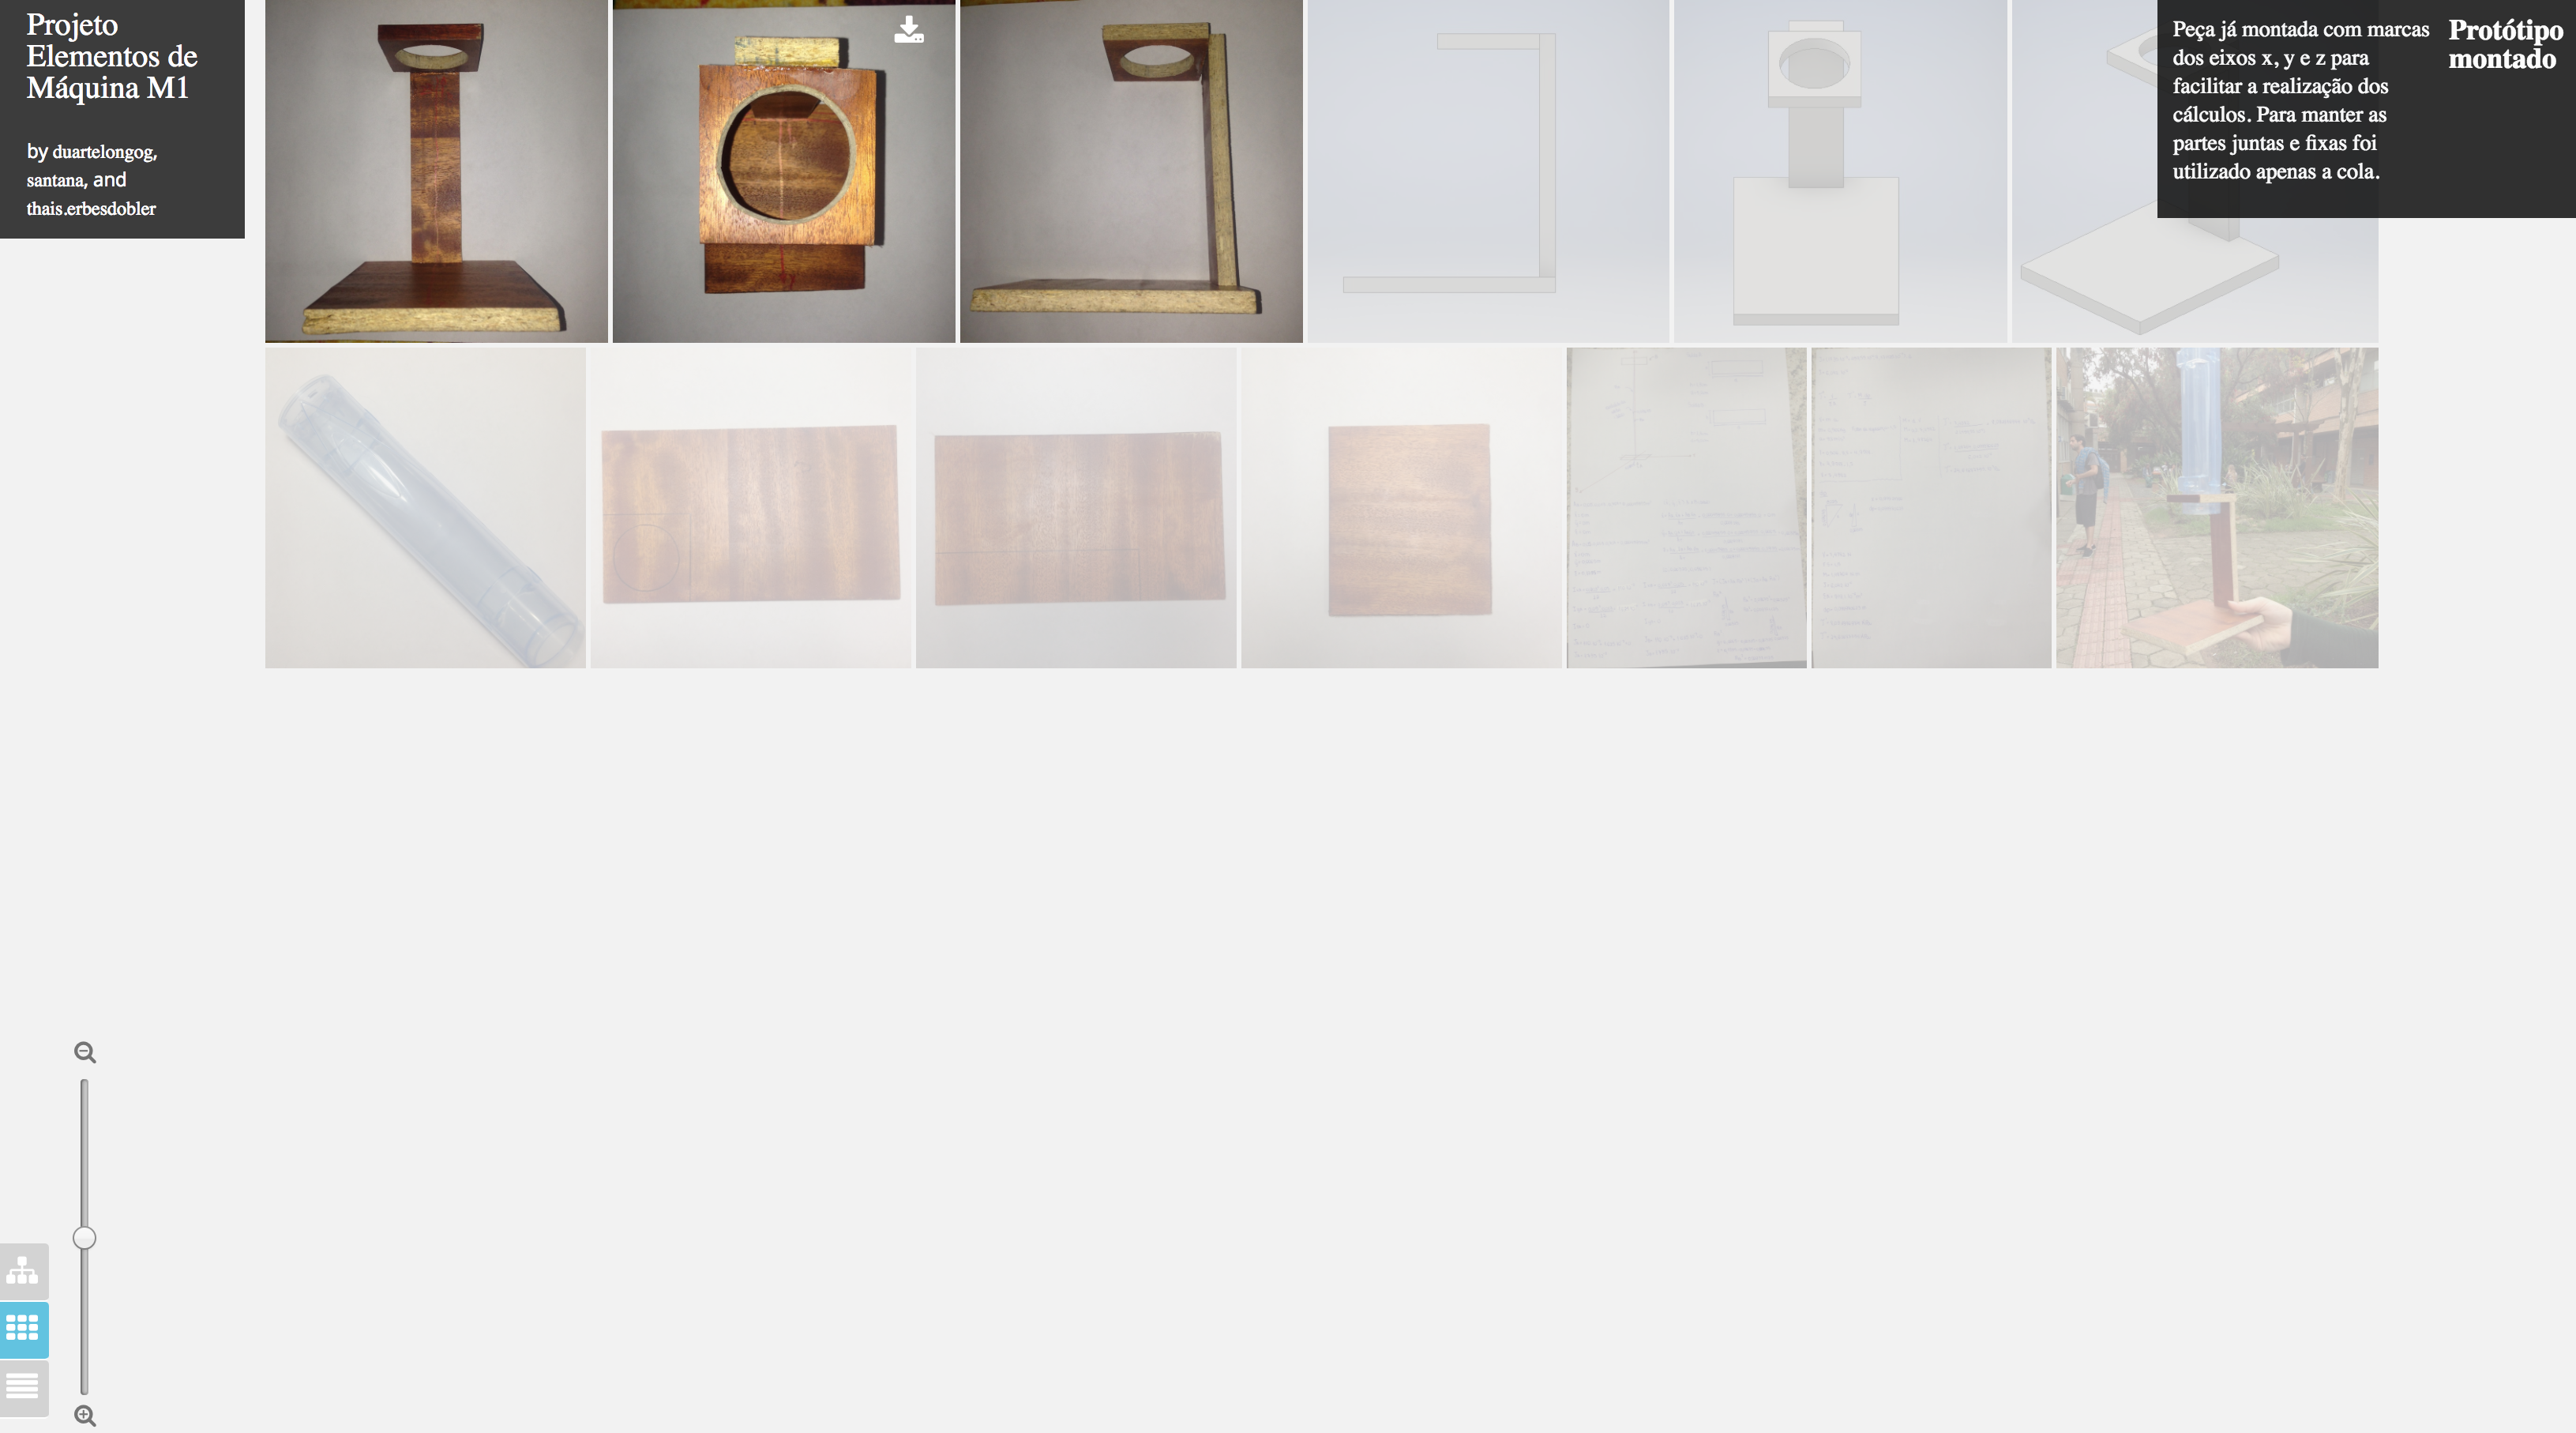
\includegraphics[scale=.16]{./images/img-mode2.png}
	\caption{Gallery view of the project} 
	\label{img-mode2}
\end{figure}

\begin{figure}[H]
	\centering
	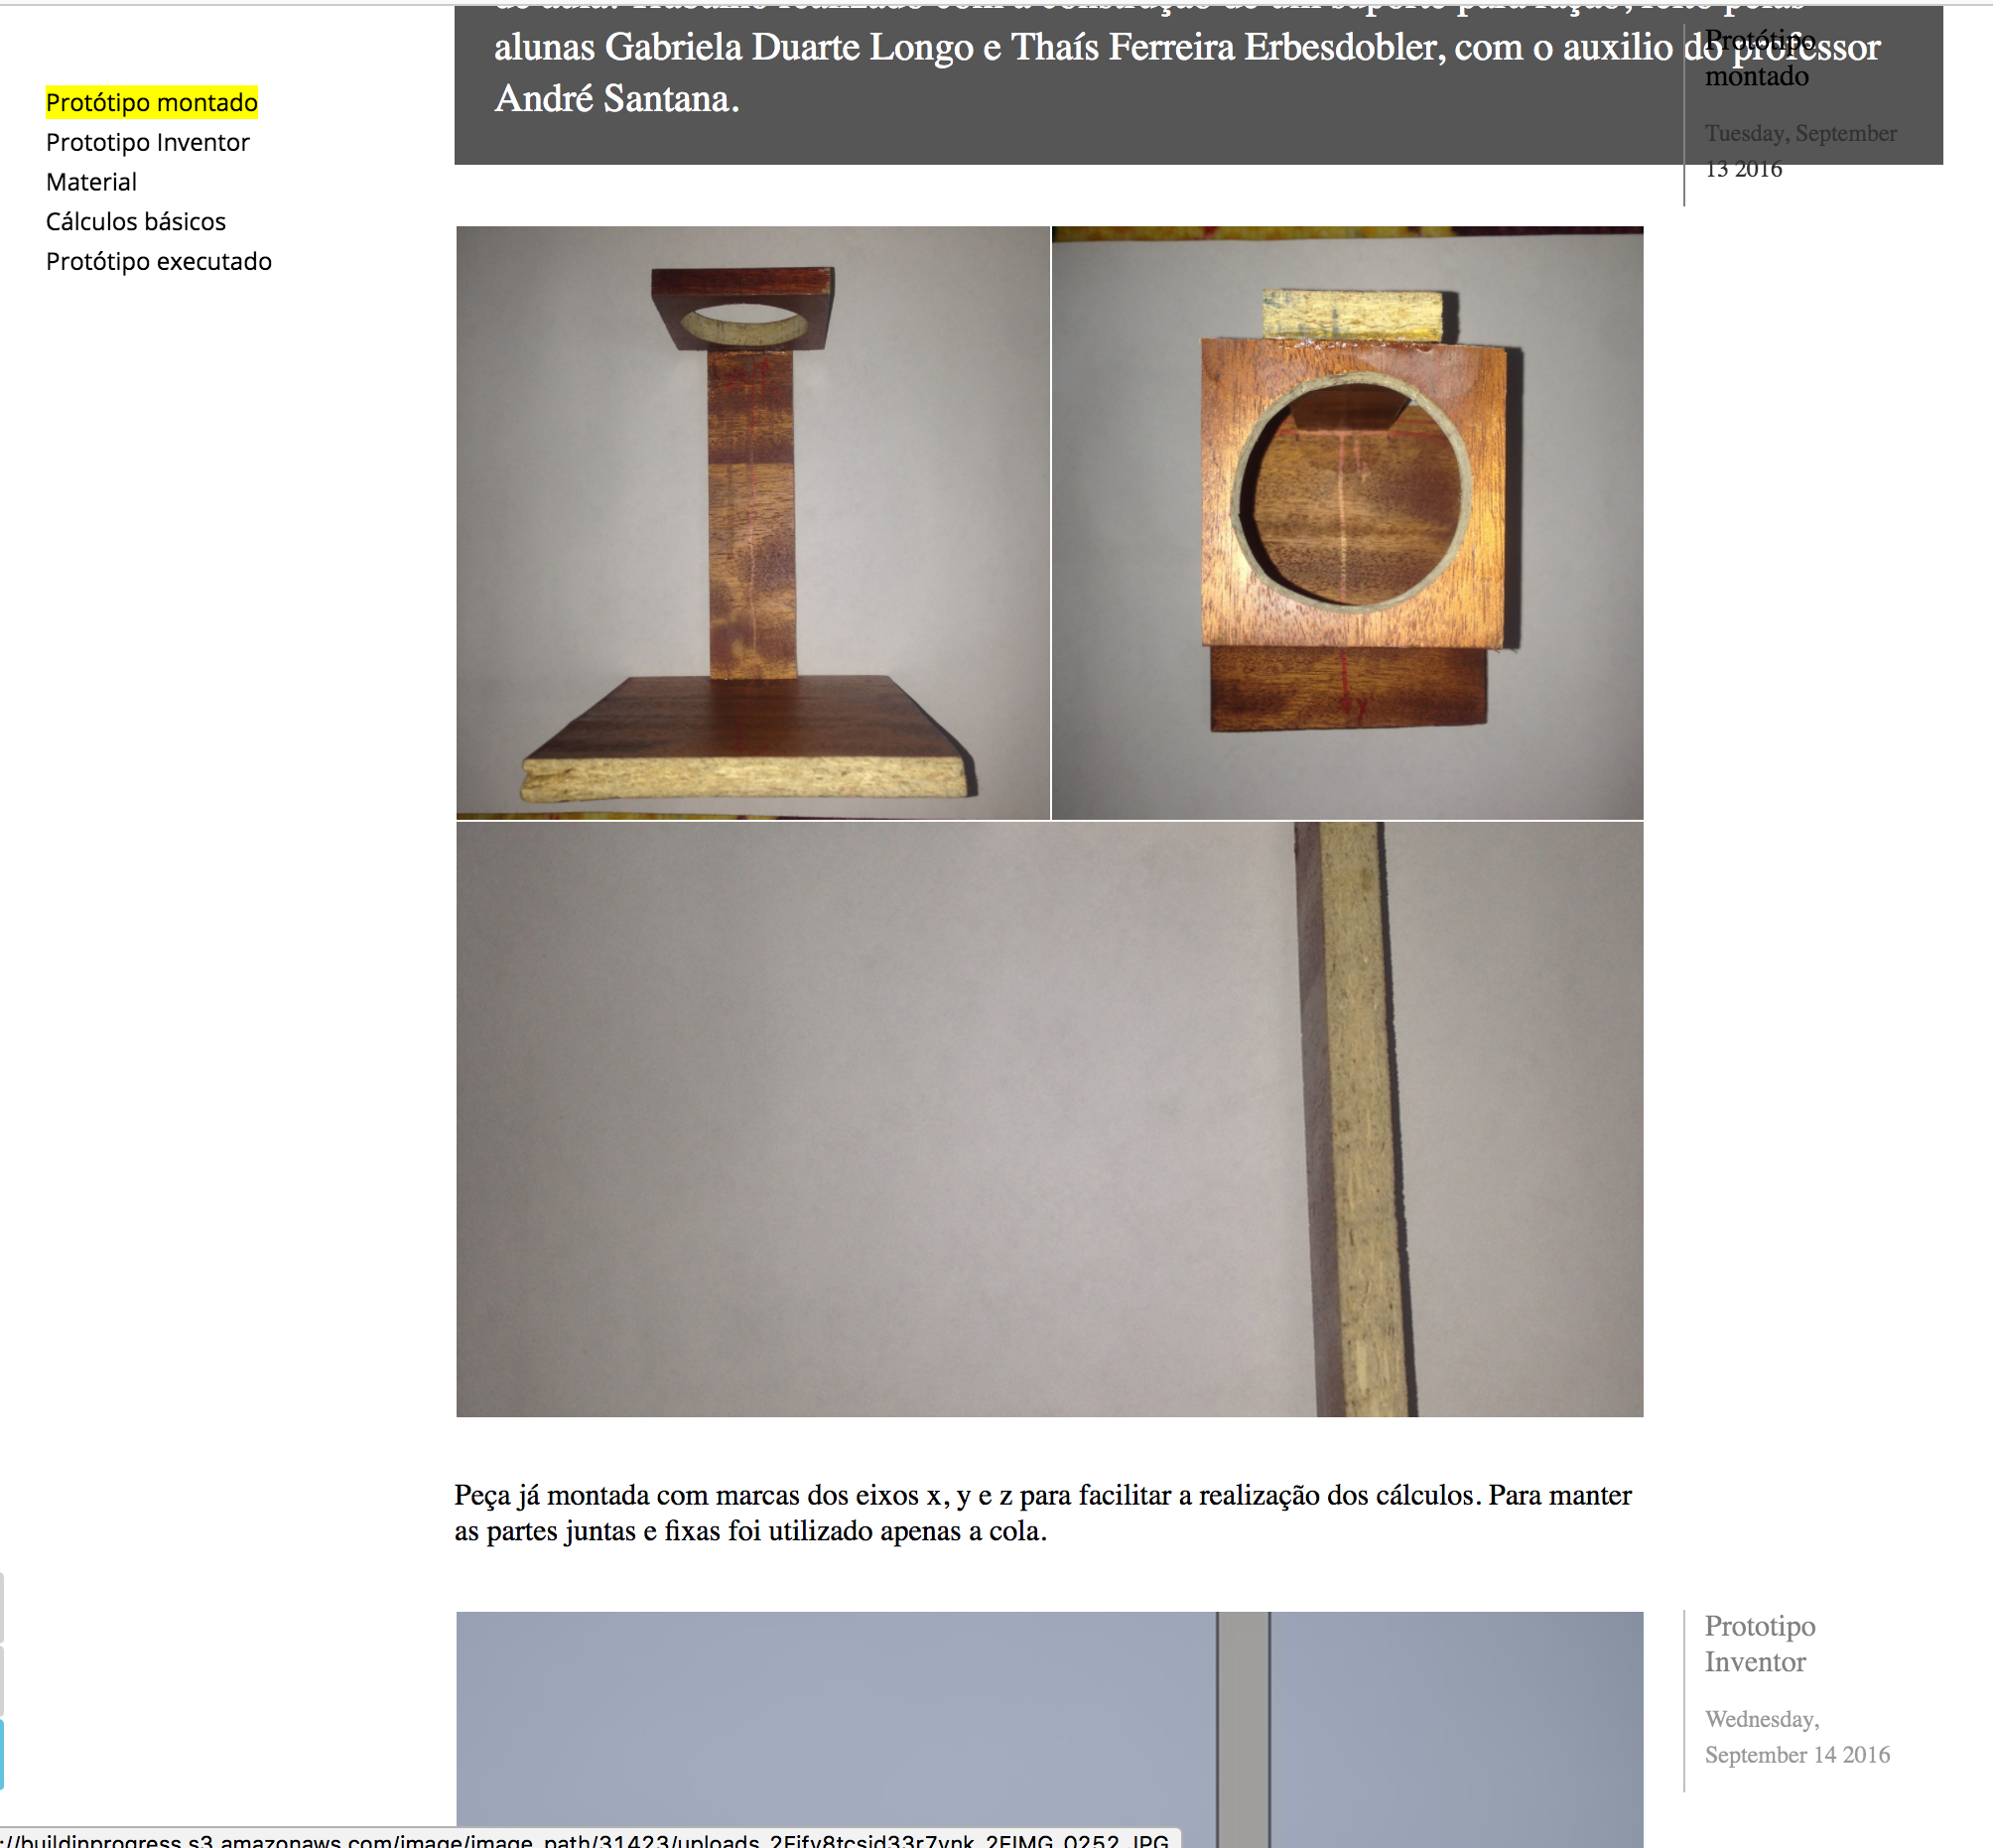
\includegraphics[scale=.3]{./images/img-mode3.png}
	\caption{Blog like mode} 
	\label{img-mode3}
\end{figure}

In \textit{Details of step} users can upload photos or videos, add text description, ask others a question that will appear in the homepage of the platform, upload resources or files in different formats; e.g. .PDF, .PPT, a given example is shown in the figure \ref{img-stepdetails} .
\begin{figure}[H]
	\centering
	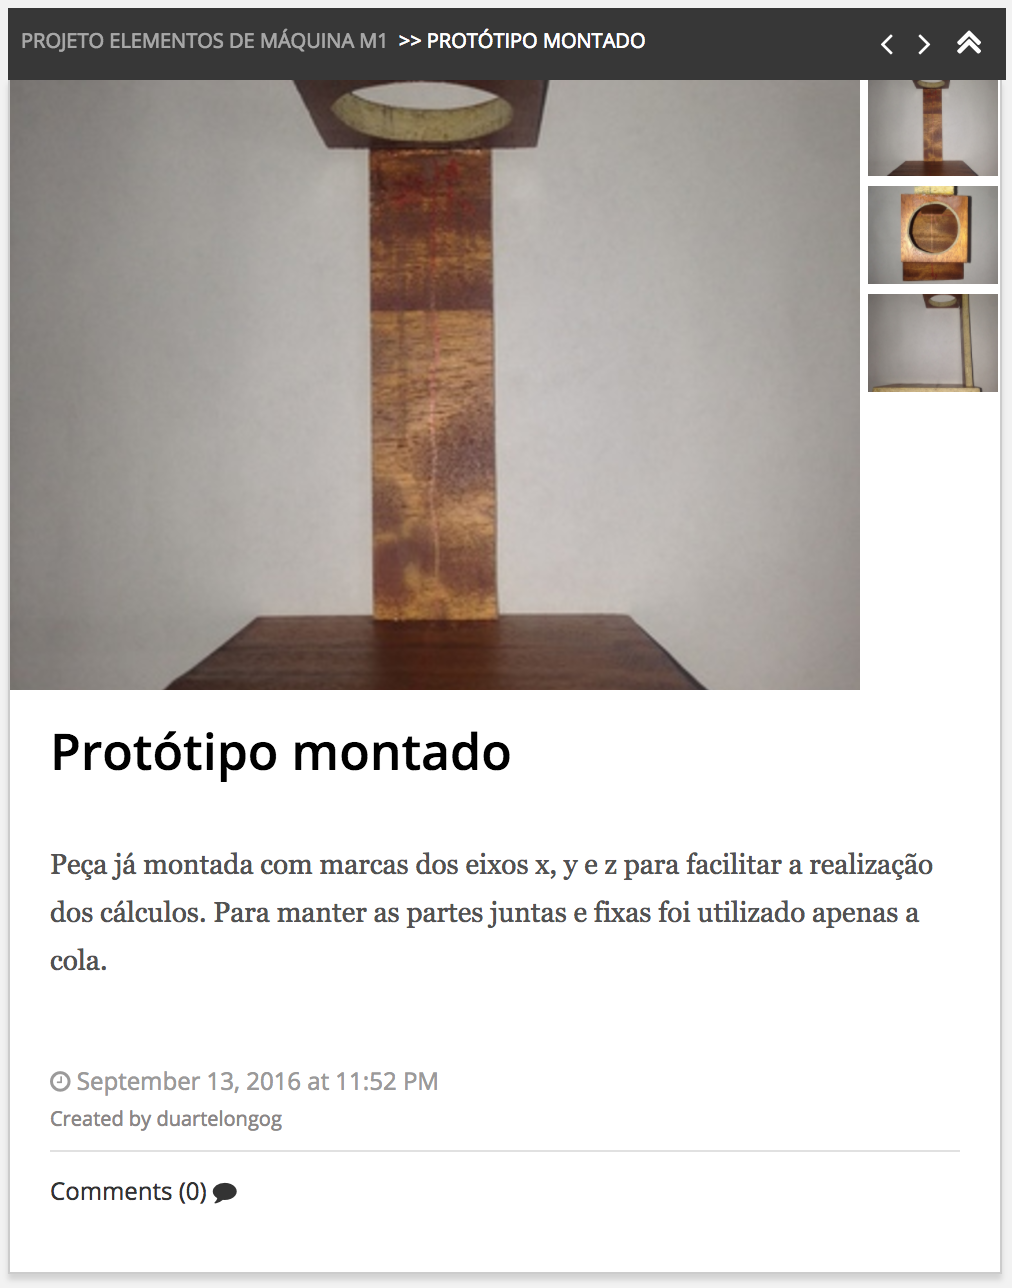
\includegraphics[scale=.3]{./images/img-stepdetails.png}
	\caption{Details steps view} 
	\label{img-stepdetails}
\end{figure}

The online platform incorporate many features that keep the BiP community more socialized and connected. Users can follow a project, see recent activity on the homepage and they will receive notification once an author add a step or ask a question.
\begin{figure}[H]
	\centering
	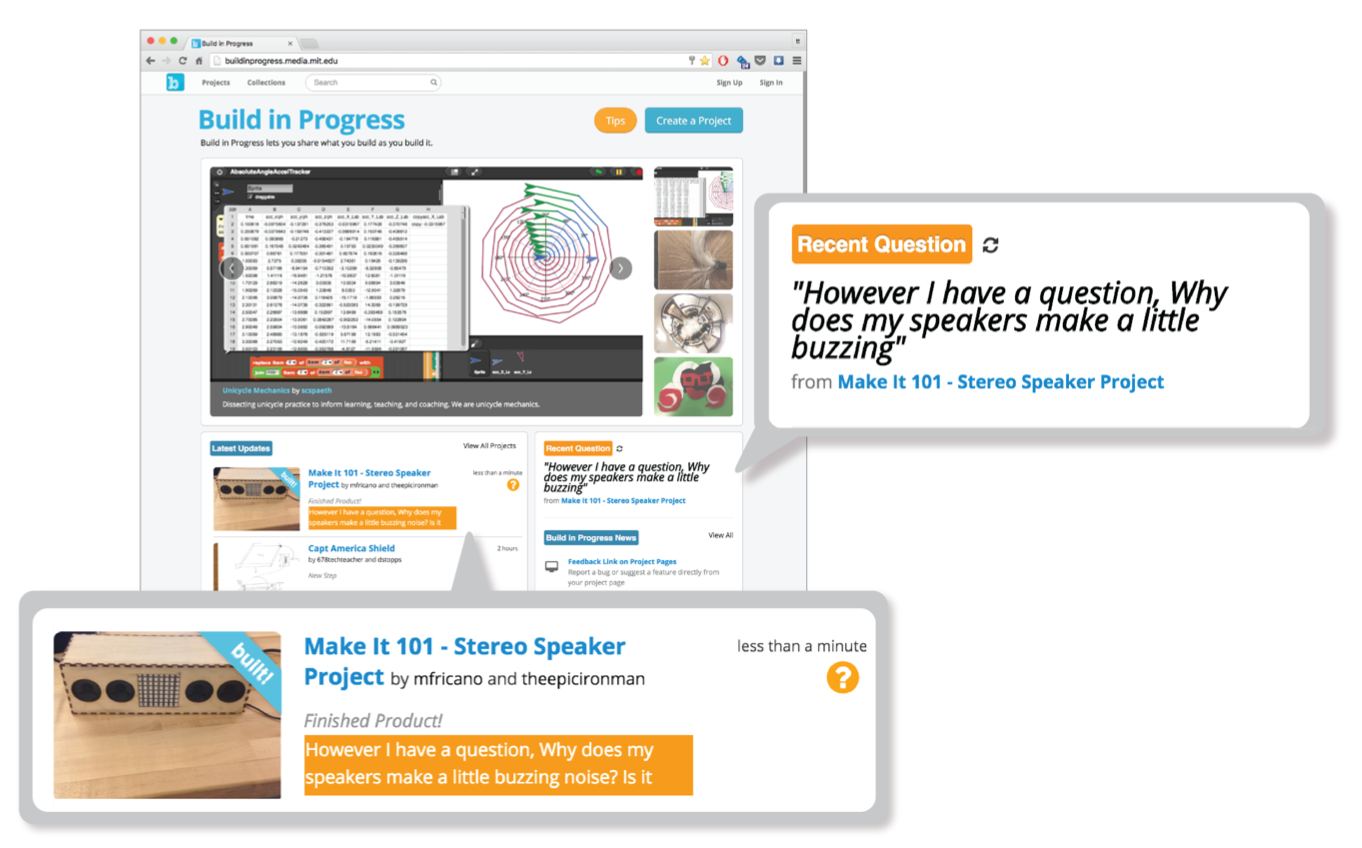
\includegraphics[scale=.4]{./images/img-commentquestion.png}
	\caption{Question featured in the home page, [Tseng, 2016]} 
	\label{img-commentquestion}
\end{figure}

Moreover, users can leave a text on any step and they will receive a notification when a comment is left. Authors can ask for feedback or help by embedding a question that will be added to the Community Activity section of the homepage, see figure \ref{img-commentquestion}.
\subsubsection{Mobile application}
A mobile application has been created to make documentation more efficient in which users upload images and videos to their projects directly from their devices instead of taking picture from their devices then transfer it to a computer and upload it (figure \ref{img-mobileapp}.
\begin{figure}[H]
	\centering
	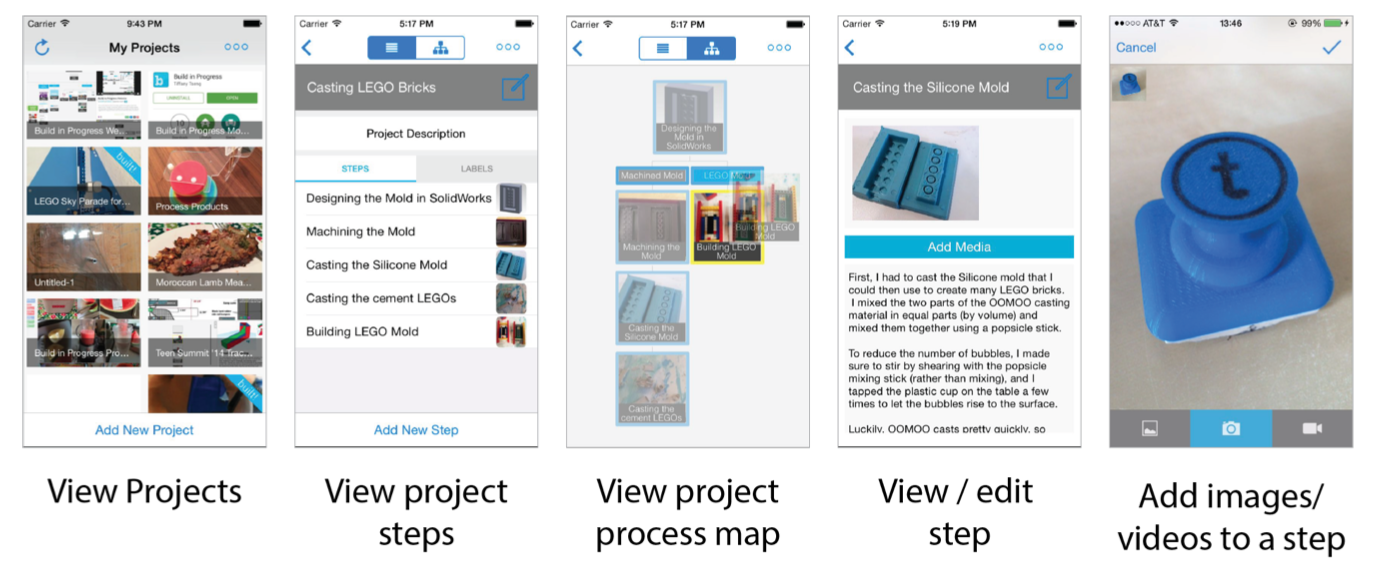
\includegraphics[scale=.5]{./images/img-mobileapp.png}
	\caption{Mobile application interface, [Tseng, 2016]} 
	\label{img-mobileapp}
\end{figure}
\subsection{User interaction}

BiP has been used in after-school  programs, in school and in workshop challenges by students and makers who work on their own project. Teenagers and one adult facilitator have been interviewed and a weekly survey was sent to all users to get an estimation about their weekly hours work.

The results of the interviews and surveys showed that users get motivated to share their project as it facilitate getting feedback, create and show their portfolio projects, get engaged to document and to help others. Users found that BiP support meaningful documentation practices and many strategies were identified depending on the type of project, the duration of a project and the age of makers who are using it.

\subsection{Summary}

The study of BuildinProgress showed that BiP support authors and readers. The documentation help makers to create a design process for their project by learning from the many iterations they did over time and BiP motivates reflective practice on making, design process, and values and identity. Users get engaged, get feedback, get self reward and help others. It support all capturing way written and visual. 



\section{Discussion}

\textit{BuildinProgress} and \textit{Instructables} didn't bring a new fundamental way in which users can share their captured media publicly or in private. Design parameters can be adjusted to support different type of users-interactions and goals.  Instructables enable users to personalize through substitution and modification of a step and any missing step mean that authors should re-create their documentation while BiP focus more on the  design process where users can iterate their project by creating new branches and forget about the unsuccessful branches.

The mix between capturing and text-based-description features in BiP enable teenagers to document. The ease of use for creating a branch, drag \& drop simplify the job for younger audience especially readers who are new to the community of \textit{DIY} as they can go through steps, iterate on their work, modify a step or re-arrange some steps.  Instructables has both features but there is no friendly structure where authors get their documentation organized and if an author has a limited background in documentation or he doesn't like it, he will probably abandon the documentation of a project after the first type a user find that it is not possible to re-arrage the documented steps.

Sharing a project is not enough for authors. Users in Instructables found that they cannot share their thought or it is limited as the only way to express what they think is via a comment. BiP offers a text-based option where both authors and readers could ask a question or leave a comment, also, both can receive a notifications for a reply from the community or any other news concerning any modification in the project.

The process of sharing the effort in progress enable users to communicate more in BiP, they helped each other, they showed their effort, they get featured and receive feedback as described in section \ref{sec:feature}. Balancing the ease of use of automated documentation systems with the powerful feature, a mobile application, encourage more users to upload pictures or videos and enable them to be physically free so they can move around to document their project for example without having the problem of taking a photo, remember which step it is, transfer it then upload it to the platform as in Instructables.

\begin{comment}

\begin{itemize}
	\item{Adapt  SDG in progress}
	
	
	\item{Qu-est ce que la platforme a apporte et ce que nous on a apporte}
	\item{Comparaison avec other platform}
	\item{ Explication about the summer school, experience, different way to document etc..} 
	\item{When we can use it and how we can use it ?} 
	
\end{itemize}


\begin{itemize}
	\item Platforme pour le soutien des hackathon grise
	\item What tiffanz said about here ieda and references
	\item securite constructif
	
	\begin{itemize}
		\item la continuite des  idess
		\item durabilitz of projects
		\item relance les projet
	\end{itemize}
	\item hackathons
	\item summer school
	\item master
	\item how to evaluate a project in time when it avaluate from team to team
	\item changement de step ou de team, continuite sachant qu'on connait des interruption forte , d'etape, d'equipe, et les 2 rests ensemble
	\item cumulative innovation
	\item in innnovation find a waz to document goodlz 
	\item rice made
	\item 
\end{itemize}

\section{IDEAS}
\begin{itemize}
	\item "Users don't want documentation, they want answers" 
\end{itemize}

\section{Features}

%% This is an example first chapter.  You should put chapter/appendix that you
%% write into a separate file, and add a line \include{yourfilename} to
%% main.tex, where `yourfilename.tex' is the name of the chapter/appendix file.
%% You can process specific files by typing their names in at the 
%% \files=
%% prompt when you run the file main.tex through LaTeX.




\label{sec:features}

The rest of this document shows off a few features of the template
files.  Look at the source code to see which macros we used!

The template is divided into \TeX{} files as follows:
\begin{enumerate}
\item \texttt{thesis.tex} is the main file.
\item \texttt{extrapackages.tex} holds extra package includes.
\item \texttt{layoutsetup.tex} defines the style used in this document.
\item \texttt{theoremsetup.tex} declares the theorem-like environments.
\item \texttt{macrosetup.tex} defines extra macros that you may find
useful.
\item \texttt{introduction.tex} contains this text.
\item \texttt{sections.tex} is a quick demo of each sectioning level
available.
\item \texttt{refs.bib} is an example bibliography file.  You can use
Bib\TeX{} to quote references.  For example, read
\cite{bringhurst1996ets} if you can get a hold of it.
\end{enumerate}


\subsection{Extra package includes}

The file \texttt{extrapackages.tex} lists some packages that usually
come in handy.  Simply have a look at the source code.  We have
added the following comments based on our experiences:
\begin{description}
\item[REC] This package is recommended.
\item[OPT] This package is optional.  It usually solves a specific
problem in a clever way.
\item[ADV] This package is for the advanced user, but solves a problem
frequent enough that we mention it. Consult the package's
documentation.
\end{description}

As a small example, here is a reference to the Section \emph{Features}
typeset with the recommended \package{varioref} package:
\begin{quote}
See Section~\vref{sec:features}.
\end{quote}


\subsection{Layout setup}

This defines the overall look of the document -- for example, it
changes the chapter and section heading appearance.  We consider this
a `do not touch' area.  Take a look at the excellent \emph{Memoir}
documentation before changing it.

In fact, take a look at the excellent \emph{Memoir} documentation,
full stop.


\subsection{Theorem setup}

This file defines a bunch of theorem-like environments.

\begin{theorem}
An example theorem.
\end{theorem}

\begin{proof}
Proof text goes here.
\end{proof}

Note that the q.e.d.\ symbol moves to the correct place automatically
if you end the proof with an \texttt{enumerate} or
\texttt{displaymath}.  You do not need to use \verb-\qedhere- as with
\package{amsthm}.

\begin{theorem}[Some Famous Guy]
Another example theorem.
\end{theorem}

\begin{proof}
This proof
\begin{enumerate}
\item ends in an enumerate.
\end{enumerate}
\end{proof}

\begin{proposition}
Note that all theorem-like environments are by default numbered on
the same counter.
\end{proposition}

\begin{proof}
This proof ends in a display like so:
\begin{displaymath}
f(x) = x^2.
\end{displaymath}
\end{proof}


\subsection{Macro setup}

For now the macro setup only shows how to define some basic macros,
and how to use a neat feature of the \package{mathtools} package:
\begin{displaymath}
\abs{a}, \quad \abs*{\frac{a}{b}}, \quad \abs[\big]{\frac{a}{b}}.
\end{displaymath}

This is version \verb-v1.4- of the template.

We assume that you found this template on our institute's website, so
we do not repeat everything stated there.  Consult the website again
for pointers to further reading about \LaTeX{}.  This chapter only
gives a brief overview of the files you are looking at.

\section{Features}
\label{sec:features}

The rest of this document shows off a few features of the template
files.  Look at the source code to see which macros we used!

The template is divided into \TeX{} files as follows:
\begin{enumerate}
\item \texttt{thesis.tex} is the main file.
\item \texttt{extrapackages.tex} holds extra package includes.
\item \texttt{layoutsetup.tex} defines the style used in this document.
\item \texttt{theoremsetup.tex} declares the theorem-like environments.
\item \texttt{macrosetup.tex} defines extra macros that you may find
useful.
\item \texttt{introduction.tex} contains this text.
\item \texttt{sections.tex} is a quick demo of each sectioning level
available.
\item \texttt{refs.bib} is an example bibliography file.  You can use
Bib\TeX{} to quote references.  For example, read
\cite{bringhurst1996ets} if you can get a hold of it.
\end{enumerate}


\subsection{Extra package includes}

The file \texttt{extrapackages.tex} lists some packages that usually
come in handy.  Simply have a look at the source code.  We have
added the following comments based on our experiences:
\begin{description}
\item[REC] This package is recommended.
\item[OPT] This package is optional.  It usually solves a specific
problem in a clever way.
\item[ADV] This package is for the advanced user, but solves a problem
frequent enough that we mention it. Consult the package's
documentation.
\end{description}

As a small example, here is a reference to the Section \emph{Features}
typeset with the recommended \package{varioref} package:
\begin{quote}
See Section~\vref{sec:features}.
\end{quote}


\subsection{Layout setup}

This defines the overall look of the document -- for example, it
changes the chapter and section heading appearance.  We consider this
a `do not touch' area.  Take a look at the excellent \emph{Memoir}
documentation before changing it.

In fact, take a look at the excellent \emph{Memoir} documentation,
full stop.


\subsection{Theorem setup}

This file defines a bunch of theorem-like environments.

\begin{theorem}
An example theorem.
\end{theorem}

\begin{proof}
Proof text goes here.
\end{proof}

Note that the q.e.d.\ symbol moves to the correct place automatically
if you end the proof with an \texttt{enumerate} or
\texttt{displaymath}.  You do not need to use \verb-\qedhere- as with
\package{amsthm}.

\begin{theorem}[Some Famous Guy]
Another example theorem.
\end{theorem}

\begin{proof}
This proof
\begin{enumerate}
\item ends in an enumerate.
\end{enumerate}
\end{proof}

\begin{proposition}
Note that all theorem-like environments are by default numbered on
the same counter.
\end{proposition}

\begin{proof}
This proof ends in a display like so:
\begin{displaymath}
f(x) = x^2.
\end{displaymath}
\end{proof}


\subsection{Macro setup}

For now the macro setup only shows how to define some basic macros,
and how to use a neat feature of the \package{mathtools} package:
\begin{displaymath}
\abs{a}, \quad \abs*{\frac{a}{b}}, \quad \abs[\big]{\frac{a}{b}}.
\end{displaymath}
\end{comment}
\chapter{Conclusion}
%\chapter{Writing scientific texts in English}

This chapter was originally a separate document written by Reto
Spöhel.  It is reprinted here so that the template can serve as a
quick guide to thesis writing, and to provide some more example
material to give you a feeling for good typesetting.

% We're going to need an extra theorem-like environment for this
% chapter
\theoremstyle{plain}
\theoremsymbol{}
\newtheorem{Rule}[theorem]{Rule}

\section{Basic writing rules}

The following rules need little further explanation; they are best
understood by looking at the example in the booklet by Knuth et al.,
§2--§3.

\begin{Rule}
  Write texts, not chains of formulas.
\end{Rule}

More specifically, write full sentences that are logically
interconnected by phrases like `Therefore', `However', `On the other
hand', etc.\ where appropriate.

\begin{Rule}
  Displayed formulas should be embedded in your text and punctuated
  with it.
\end{Rule}

In other words, your writing should not be divided into `text parts'
and `formula parts'; instead the formulas should be tied together by
your prose such that there is a natural flow to your writing.

\section{Being nice to the reader}

Try to write your text in such a way that a reader enjoys reading
it. That's of course a lofty goal, but nevertheless one you should
aspire to!

\begin{Rule}
  Be nice to the reader.
\end{Rule}

Give some intuition or easy example for definitions and theorems which
might be hard to digest. Remind the reader of notations you introduced
many pages ago -- chances are he has forgotten them. Illustrate your
writing with diagrams and pictures where this helps the reader. Etc.

\begin{Rule}
  Organize your writing.
\end{Rule}

Think carefully about how you subdivide your thesis into chapters,
sections, and possibly subsections.  Give overviews at the beginning
of your thesis and of each chapter, so the reader knows what to
expect. In proofs, outline the main ideas before going into technical
details. Give the reader the opportunity to `catch up with you' by
summing up your findings periodically.

\emph{Useful phrases:} `So far we have shown that \ldots', `It remains
to show that \ldots', `Recall that we want to prove inequality (7), as
this will allow us to deduce that \ldots', `Thus we can conclude that
\ldots. Next, we would like to find out whether \ldots', etc.

\begin{Rule}
  Don't say the same thing twice without telling the reader that you
  are saying it twice.
\end{Rule}

Repetition of key ideas is important and helpful. However, if you
present the same idea, definition or observation twice (in the same or
different words) without telling the reader, he will be looking for
something new where there is nothing new.

\emph{Useful phrases:} `Recall that [we have seen in Chapter 5 that]
\ldots', `As argued before / in the proof of Lemma 3, \ldots', `As
mentioned in the introduction, \ldots', `In other words, \ldots', etc.

\begin{Rule}
  Don't make statements that you will justify later without telling
  the reader that you will justify them later.
\end{Rule}

This rule also applies when the justification is coming right in the
next sentence!  The reasoning should be clear: if you violate it, the
reader will lose valuable time trying to figure out on his own what
you were going to explain to him anyway.

\emph{Useful phrases:} `Next we argue that \ldots', `As we shall see,
\ldots', `We will see in the next section that \ldots, etc.


\section{A few important grammar rules}

\begin{Rule}
  \label{rule:no-comma-before-that}
  There is (almost) \emph{never} a comma before `that'.
\end{Rule}

It's really that simple. Examples:
\begin{quote}
  We assume that \ldots\\
  \emph{Wir nehmen an, dass \ldots}

  It follows that \ldots\\
  \emph{Daraus folgt, dass \ldots}

  `thrice' is a word that is seldom used.\\
  \emph{`thrice' ist ein Wort, das selten verwendet wird.}
\end{quote}
Exceptions to this rule are rare and usually pretty obvious. For
example, you may end up with a comma before `that' because `i.e.' is
spelled out as `that is':
\begin{quote}
  For \(p(n)=\log n/n\) we have \ldots{} However, if we choose \(p\) a
  little bit higher, that is \(p(n)=(1+\varepsilon)\log n/n\) for some
  \(\varepsilon>0\), we obtain that\ldots
\end{quote}
Or you may get a comma before `that' because there is some additional
information inserted in the middle of your sentence:
\begin{quote}
  Thus we found a number, namely \(n_0\), that satisfies equation (13).
\end{quote}
If the additional information is left out, the sentence has no comma:
\begin{quote}
  Thus we found a number that satisfies equation (13).
\end{quote}
(For `that' as a relative pronoun, see also
Rules~\ref{rule:non-defining-has-comma}
and~\ref{rule:defining-without-comma} below.)

\begin{Rule}
  There is usually no comma before `if'.
\end{Rule}

Example:
\begin{quote}
  A graph is not \(3\)-colorable if it contains a \(4\)-clique.\\
  \emph{Ein Graph ist nicht \(3\)-färbbar, wenn er eine \(4\)-Clique
    enthält.}
\end{quote}
However, if the `if' clause comes first, it is usually separated from
the main clause by a comma:
\begin{quote}
  If a graph contains a \(4\)-clique, it is not \(3\)-colorable .\\
  \emph{Wenn ein Graph eine \(4\)-Clique enthält, ist er nicht
    \(3\)-färbbar.}
\end{quote}

There are more exceptions to these rules than to
Rule~\ref{rule:no-comma-before-that}, which is why we are not
discussing them here. Just keep in mind: don't put a comma before `if'
without good reason.

\begin{Rule}
  \label{rule:non-defining-has-comma}
  Non-defining relative clauses have commas.
\end{Rule}
\begin{Rule}
  \label{rule:defining-without-comma}
  Defining relative clauses have no commas.
\end{Rule}

In English, it is very important to distinguish between two types of
relative clauses: defining and non-defining ones. This is a
distinction you absolutely need to understand to write scientific
texts, because mistakes in this area actually distort the meaning of
your text!

It's probably easier to explain first what a \emph{non-defining}
relative clause is. A non-defining relative clauses simply gives
additional information \emph{that could also be left out} (or given in
a separate sentence). For example, the sentence
\begin{quote}
  The \textsc{WeirdSort} algorithm, which was found by the famous
  mathematician John Doe, is theoretically best possible but difficult
  to implement in practice.
\end{quote}
would be fully understandable if the relative clause were left out
completely. It could also be rephrased as two separate sentences:
\begin{quote}
  The \textsc{WeirdSort} algorithm is theoretically best possible but
  difficult to implement in practice. [By the way,] \textsc{WeirdSort}
  was found by the famous mathematician John Doe.
\end{quote}
This is what a non-defining relative clause is. \emph{Non-defining
  relative clauses are always written with commas.} As a corollary we
obtain that you cannot use `that' in non-defining relative clauses
(see Rule~\ref{rule:no-comma-before-that}!). It would be wrong to
write
\begin{quote}
  \st{The \textsc{WeirdSort} algorithm, that was found by the famous
    mathematician John Doe, is theoretically best possible but
    difficult to implement in practice.}
\end{quote}
A special case that warrants its own example is when `which' is
referring to the entire preceding sentence:
\begin{quote}
  Thus inequality (7) is true, which implies that the Riemann
  hypothesis holds.
\end{quote}
As before, this is a non-defining relative sentence (it could be left
out) and therefore needs a comma.

So let's discuss \emph{defining} relative clauses next. A defining
relative clause tells the reader \emph{which specific item the main
  clause is talking about}. Leaving it out either changes the meaning
of the sentence or renders it incomprehensible altogether.  Consider
the following example:

\begin{quote}
  The \textsc{WeirdSort} algorithm is difficult to implement in
  practice. In contrast, the algorithm that we suggest is very simple.
\end{quote}

Here the relative clause `that we suggest' cannot be left out -- the
remaining sentence would make no sense since the reader would not know
which algorithm it is talking about. This is what a defining relative
clause is. \textit{Defining relative clauses are never written with
  commas.} Usually, you can use both `that' and `which' in defining
relative clauses, although in many cases `that' sounds better.

As a final example, consider the following sentence:
\begin{quote}
  For the elements in \(\mathcal{B}\) which satisfy property (A), we
  know that equation (37) holds.
\end{quote}
This sentence does not make a statement about all elements in
\(\mathcal{B}\), only about those satisfying property (A). The relative
clause is \emph{defining}. (Thus we could also use `that' in place of
`which'.)

In contrast, if we add a comma the sentence reads
\begin{quote}
  For the elements in \(\mathcal{B}\), which satisfy property (A), we
  know that equation (37) holds.
\end{quote}

Now the relative clause is \emph{non-defining} -- it just mentions in
passing that all elements in \(\mathcal{B}\) satisfy property (A). The
main clause states that equation (37) holds for \emph{all} elements in
\(\mathcal{B}\). See the difference?


\section[Things you (usually) don't say in English]%
{Things you (usually) don't say in English -- and what to say
  instead}
\label{sec:list}

Table~\ref{tab:things-you-dont-say} lists some common mistakes and
alternatives.  The entries should not be taken as gospel -- they don't
necessarily mean that a given word or formulation is wrong under all
circumstances (obviously, this depends a lot on the context). However,
in nine out of ten instances the suggested alternative is the better
word to use.

\begin{table}
  \centering
  \caption{Things you (usually) don't say}
  \label{tab:things-you-dont-say}
  \begin{tabular}{lll}
    \toprule
    \st{It holds (that) \dots} & We have \dots & \emph{Es gilt \dots}\\
    \multicolumn{3}{l}{\quad\footnotesize(`Equation (5) holds.' is fine, though.)}\\
    \st{$x$ fulfills property $\mathcal{P}$.}& \(x\) satisfies property \(\mathcal{P}\). & \emph{\(x\) erfüllt Eigenschaft \(\mathcal{P}\).} \\
    \st{in average} & on average & \emph{im Durchschnitt}\\
    \st{estimation} & estimate   & \emph{Abschätzung}\\
    \st{composed number} & composite number & \emph{zusammengesetzte Zahl}\\
    \st{with the help of} & using & \emph{mit Hilfe von}\\
    \st{surely} & clearly & \emph{sicher, bestimmt}\\
    \st{monotonously increasing} & monotonically incr. & \emph{monoton steigend}\\
    \multicolumn{3}{l}{\quad\footnotesize(Actually, in most cases `increasing' is just fine.)}\\
    \bottomrule
  \end{tabular}
\end{table}

%%% Local Variables:
%%% mode: latex
%%% TeX-master: "thesis"
%%% End:

%\chapter{Typography}


\section{Punctuation}

\begin{Rule}
  Use opening (`) and closing (') quotation marks correctly.
\end{Rule}

In \LaTeX, the closing quotation mark is typed like a normal
apostrophe, while the opening quotation mark is typed using the French
\emph{accent grave} on your keyboard (the \emph{accent grave} is the
one going down, as in \emph{frère}).

Note that any punctuation that \emph{semantically} follows quoted
speech goes inside the quotes in American English, but outside in
Britain.  Also, Americans use double quotes first.  Oppose
\begin{quote}
  ``Using `lasers,' we punch a hole in \ldots\ the Ozone Layer,''
  Dr.\ Evil said.
\end{quote}
to
\begin{quote}
  `Using ``lasers'', we punch a hole in \ldots\ the Ozone Layer',
  Dr.\ Evil said.
\end{quote}

\begin{Rule}
  Use hyphens (-), en-dashes (--) and em-dashes (---) correctly.
\end{Rule}

A hyphen is only used in words like `well-known', `$3$-colorable'
etc., or to separate words that continue in the next line (which is
known as hyphenation).  It is entered as a single ASCII hyphen
character (\texttt{-}).

To denote ranges of numbers, chapters, etc., use an en-dash (entered
as two ASCII hyphens \texttt{--}) with no spaces on either side.  For
example, using Equations (1)--(3), we see\ldots

As the equivalent of the German \emph{Gedankenstrich}, use an en-dash
with spaces on both sides -- in the title of Section \ref{sec:list},
it would be wrong to use a hyphen instead of the dash. (Some English
authors use the even longer emdash (---) instead, which is typed as
three subsequent hyphens in \LaTeX. This emdash is used without spaces
around it---like so.)


\section{Spacing}

\begin{Rule}
  \label{rule:no-manual-spacing}
  Do not add spacing manually.
\end{Rule}

You should never use the commands \lstinline-\\- (except within
tabulars and arrays), \lstinline[showspaces=true]-\ - (except to
prevent a sentence-ending space after Dr.\ and such),
\lstinline-\vspace-, \lstinline-\hspace-, etc.  The choices programmed
into \LaTeX{} and this style should cover almost all cases.  Doing it
manually quickly leads to inconsistent spacing, which looks terrible.
Note that this list of commands is by no means conclusive.

\begin{Rule}
  Judiciously insert spacing in maths where it helps.
\end{Rule}

This directly contradicts Rule~\ref{rule:no-manual-spacing}, but in
some cases \TeX{} fails to correctly decide how much spacing is
required.  For example, consider
\begin{displaymath}
  f(a,b) = f(a+b, a-b).
\end{displaymath}
In such cases, inserting a thin math space \lstinline-\,- greatly
increases readability:
\begin{displaymath}
  f(a,b) = f(a+b,\, a-b).
\end{displaymath}

Along similar lines, there are variations of some symbols with
different spacing.  For example, Lagrange's Theorem states that
\(\abs{G}=[G:H]\abs{H}\), but the proof uses a bijection \(f\colon
aH\to bH\).  (Note how the first colon is symmetrically spaced, but
the second is not.)

\begin{Rule}
  Learn when to use \lstinline[showspaces=true]-\ - and
  \lstinline-\@-.
\end{Rule}

Unless you use `french spacing', the space at the end of a sentence is
slightly larger than the normal interword space.

The rule used by \TeX{} is that any space following a period,
exclamation mark or question mark is sentence-ending, except for
periods preceded by an upper-case letter.  Inserting \lstinline-\-
before a space turns it into an interword space, and inserting
\lstinline-\@- before a period makes it sentence-ending.  This means
you should write
\begin{lstlisting}
Prof.\ Dr.\ A. Steger is a member of CADMO\@.
If you want to write a thesis with her, you
should use this template.
\end{lstlisting}
which turns into
\begin{quote}
  Prof.\ Dr.\ A. Steger is a member of CADMO\@.  If you want to write
  a thesis with her, you should use this template.
\end{quote}
The effect becomes more dramatic in lines that are stretched slightly
during justification:
\begin{quote}
  \parbox{\linewidth}{\hbox to \linewidth{%
      Prof.\ Dr.\ A. Steger is a member of CADMO\@.  If you}}
\end{quote}

\begin{Rule}
  Place a non-breaking space (\lstinline-~-) right before references.
\end{Rule}

This is actually a slight simplification of the real rule, which
should invoke common sense.  Place non-breaking spaces where a line
break would look `funny' because it occurs right in the middle of a
construction, especially between a reference type (Chapter) and its
number.


\section{Choice of `fonts'}

Professional typography distinguishes many font attributes, such as
family, size, shape, and weight.  The choice for sectional divisions
and layout elements has been made, but you will still occasionally
want to switch to something else to get the reader's attention.  The
most important rule is very simple.

\begin{Rule}
  When emphasising a short bit of text, use \lstinline-\emph-.
\end{Rule}

In particular, \emph{never} use bold text (\lstinline-\textbf-).
Italics (or Roman type if used within italics) avoids distracting the
eye with the huge blobs of ink in the middle of the text that bold
text so quickly introduces.

Occasionally you will need more notation, for example, a consistent
typeface used to identify algorithms.

\begin{Rule}
  Vary one attribute at a time.
\end{Rule}

For example, for \textsc{WeirdSort} we only changed the shape to small
caps.  Changing two attributes, say, to bold small caps would be
excessive (\LaTeX{} does not even have this particular variation).
The same holds for mathematical notation: the reader can easily
distinguish \(g_n\), \(G(x)\), \(\mathcal{G}\) and \(\mathsf{G}\).

\begin{Rule}
  Never underline or uppercase.
\end{Rule}

No exceptions to this one, unless you are writing your thesis on a
typewriter.  Manually.  Uphill both ways.  In a blizzard.


\section{Displayed equations}

\begin{Rule}
  Insert paragraph breaks \emph{after} displays only where they
  belong.  Never insert paragraph breaks \emph{before} displays.
\end{Rule}

\LaTeX{} translates sequences of more than one linebreak (i.e., what
looks like an empty line in the source code) into a paragraph break in
almost all contexts.  This also happens before and after displays,
where extra spacing is inserted to give a visual indication of the
structure.  Adding a blank line in these places may look nice in the
sources, but compare the resulting display

\begin{displaymath}
  a = b
\end{displaymath}

to the following:
\begin{displaymath}
  a = b
\end{displaymath}
The first display is surrounded by blank lines, but the second is not.
It is bad style to start a paragraph with a display (you should always
tell the reader what the display means first), so the rule follows.

\begin{Rule}
  Never use \lstinline-eqnarray-.
\end{Rule}

It is at the root of most ill-spaced multiline displays.  The
\package{amsmath} package provides better alternatives, such as the
\lstinline-align- family
\begin{align*}
  f(x) &= \sin x, \\
  g(x) &= \cos x,
\end{align*}
and \lstinline-multline- which copes with excessively long equations:
\begin{multline*}
  \def\P{\mathrm P}
  \P\bigl[X_{t_0} \in (z_0, z_0+dz_0],\ldots, X_{t_n}\in(z_n,z_n+dz_n]\bigr]
  \\= \nu(dz_0) K_{t_1}(z_0,dz_1) K_{t_2-t_1}(z_1,dz_2)\cdots
  K_{t_n-t_{n-1}}(z_{n-1},dz_n).
\end{multline*}


\section{Floats}

By default this style provides floating environments for tables and
figures.  The general structure should be as follows:
\begin{lstlisting}
\begin{figure}
  \centering
  % content goes here
  \caption{A short caption}
  \label{some-short-label}
\end{figure}
\end{lstlisting}
Note that the label must follow the caption, otherwise the label will
refer to the surrounding section instead.  Also note that figures
should be captioned at the bottom, and tables at the top.

The whole point of floats is that they, well, \emph{float} to a place
where they fit without interrupting the text body.  This is a frequent
source of confusion and changes; please leave it as is.

\begin{Rule}
  Do not restrict float movement to only `here'
  \textnormal{(\lstinline-h-)}.
\end{Rule}

If you are still tempted, you should avoid the float altogether and
just show the figure or table inline, similar to a displayed equation.

%%% Local Variables:
%%% mode: latex
%%% TeX-master: "thesis"
%%% End:

%\chapter{Example Chapter}

Dummy text.

\section{Example Section}

Dummy text.

\subsection{Example Subsection}

Dummy text.

\subsubsection{Example Subsubsection}

Dummy text.

\paragraph{Example Paragraph}

Dummy text.

\subparagraph{Example Subparagraph}

Dummy text.


\appendix

%\chapter{Dummy Appendix}

You can defer lengthy calculations that would otherwise only interrupt
the flow of your thesis to an appendix.


\backmatter
\bibliography{refs}
\bibliographystyle{apalike}
%\bibliographystyle{plain}


%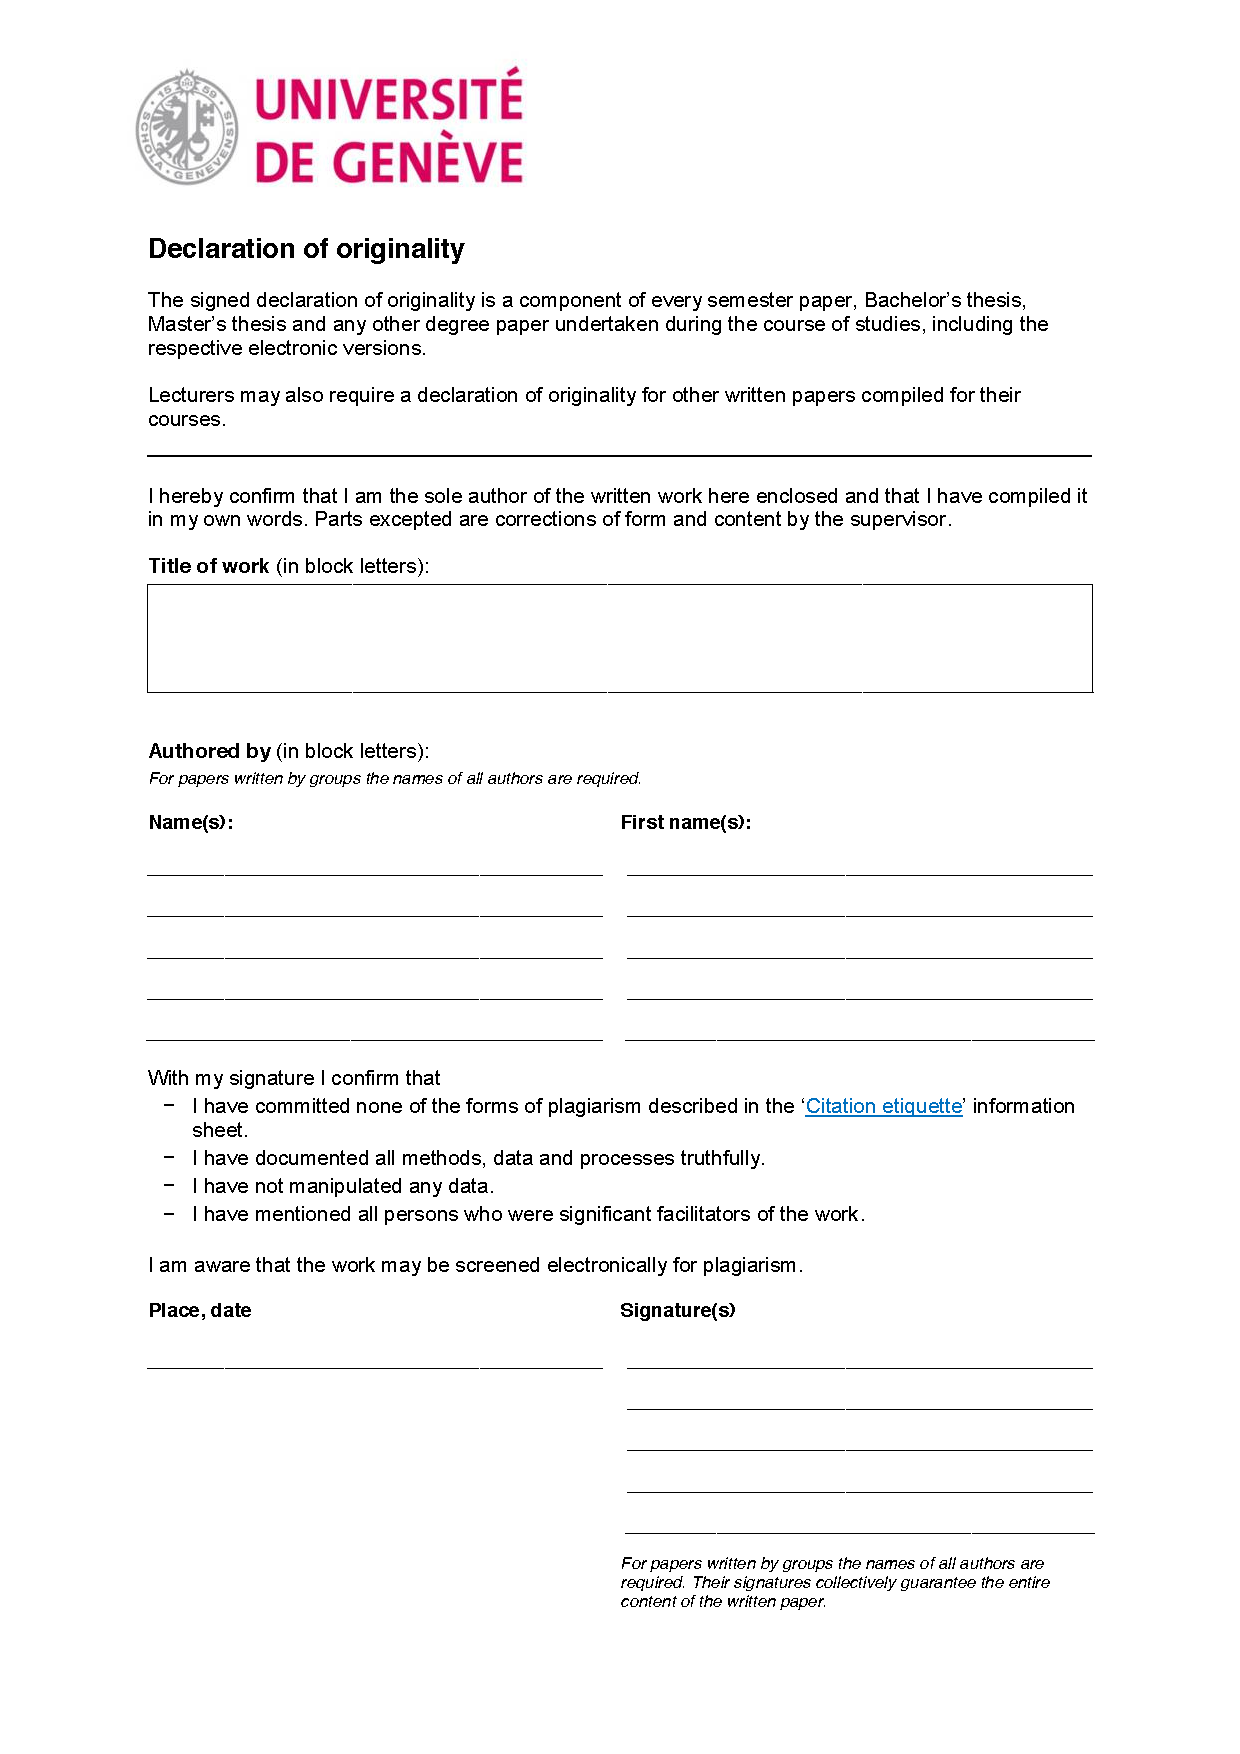
\includepdf[pages={-}]{declaration-originality.pdf}

\end{document}
